\chapter{Hiện thực hệ thống}
\section{Module nhận diện làn đường}
Nhận dạng, xác định làn đường đối các thiết bị tự hành (Autonomous vehicles) cũng như các hệ thống hỗ trợ lái xe (Driver Assistance Systems) là bài toán đặc biệt quan trong, đòi hỏi ngày càng cao về sự chính xác, an toàn ngay cả trong nhiều điều kiện khác nhau như ánh sáng, thời tiết thay đổi, sự đa dạng về môi trường hoạt động. Đối với các thiết
bị tự hành trong công nghiệp trước đây, dữ liệu đầu vào thường lấy từ các cảm biến như cảm biến hồng ngoại, cảm biến từ trường... cùng với những thiết kế cố định đối với môi trường hoạt động như ánh sáng, line đường..., điều đó làm giới hạn phạm vi hoạt động cũng như tính đa dụng của các thiết bị. Những thiết bị tự hành hiện đại hiện nay như ô tô không người lái, máy bay không người lái, robot vận chuyển hàng hóa, drone giao
hàng tự động thường sử dụng các hệ thống camera để thu thập dữ liệu cho việc xác định quỹ đạo di chuyển. Dữ liệu của camera sẽ được xử lý bằng các thuật toán xử lý ảnh hoặc các mô hình học sâu
\subsection{Các công trình liên quan}
\subsubsection{Thuật toán xử lý ảnh thông thường}
Dữ liệu từ cảm biến camera có thể được xử lý bằng các thuật toán xử lý ảnh thông thường như loc màu, phát hiện cạnh, xoay ảnh, loc nhiễu... để bóc tách được các line đường từ đó xác định được làn đường và tâm đường.
\newpage
\begin{figure}[!hbt]
\begin{center}
    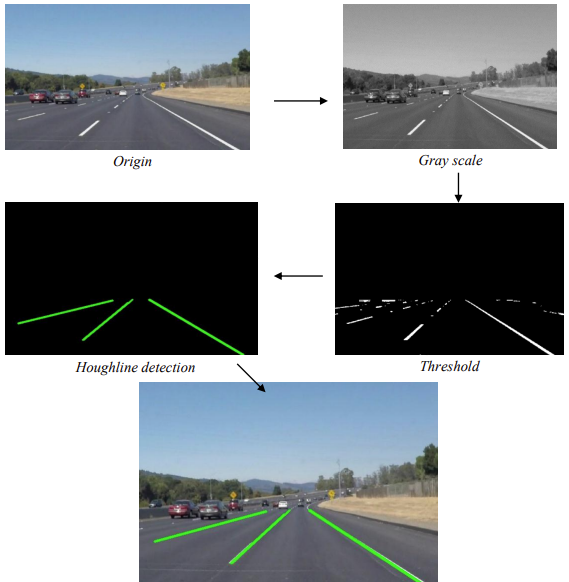
\includegraphics[width=14cm]{img/4_Implement/opencv_stages.png}
    \caption{Các giai đoạn xử lý ảnh lọc xác định làn đường sử dụng camera}
\end{center}
\end{figure}
Tuy nhiên, những thuật toán đó thường thiếu ổn định với nhiễu do độ sáng thay đổi, làn đường xuất hiện bóng cây, làn đường bị mưa ướt và thậm chí không thể xác định được làn đường khi line đường bị mất
\subsubsection{Kiến trúc học sâu}
\subsubsection{Đánh giá các model nhận diện làn đường}
Để chọn được model nhận diện làn đường phù hợp, nhóm sẽ đánh giá hiệu suất của các model khác nhau. Mục tiêu là đánh giá độ chính xác, tốc độ và độ ổn định của chúng.\\
\noindent Tập dữ liệu BDD100K\textsuperscript{\cite{bdd100k}} được sử dụng để train và đánh giá các model. Tập dữ liệu sẽ được chia thành ba phần: tập train với 70.000 ảnh, tập xác thực với 10.000 ảnh và tập đánh giá với 20.000 ảnh. Các hình ảnh sẽ được thay đổi kích thước từ 1280 × 720 xuống còn 640 × 360. Tất cả các thí nghiệm đều sử dụng framework PyTorch trên GPU NVIDIA GeForce RTX 4080.\\
\begin{table}[!hbt]
\begin{center}
\begin{tabular}{@{}cccc@{}}
\toprule
\textbf{Model} & \textbf{Kích thước} & \textbf{Params} & \textbf{Tốc độ (fps)} \\ \midrule
YOLOP\textsuperscript{\cite{yolop}}          & 640           & 7.9M            & 37                   \\
HybridNets\textsuperscript{\cite{hybridnets}}     & 640           & 12.8M           & 18                   \\
YOLOPv2\textsuperscript{\cite{yolopv2}}        & 640           & 38.9M           & 83                   \\ \midrule
TwinLiteNet\textsuperscript{\cite{twinlitenet}}    & 640           & \textbf{0.4M}   & \textbf{271}         \\ \bottomrule
\end{tabular}
\caption{\label{param-fps-table}Trọng số và tốc độ dự đoán của model}
\end{center}
\end{table}\\
Bảng \ref{param-fps-table} so sánh model TwinLiteNet \textsuperscript{\cite{twinlitenet}} với các model khác. TwinLiteNet chỉ có 0.4 triệu trọng số, ít hơn nhiều so với các model trước đây. Ngoài ra, TwinLiteNet còn đạt được 271 FPS, trong khi các model khác chỉ đạt được tốc độ dự đoán dưới 100 FPS trên cùng thiết bị.\\
\begin{table}[!hbt]
\begin{center}
\begin{tabular}{@{}ccc@{}}
\toprule
\textbf{Model} & \textbf{Độ chính xác (\%)} & \textbf{IoU (\%)} \\ \midrule
Enet\textsuperscript{\cite{enet}}                 & 34.12                      & 14.64             \\
SCNN\textsuperscript{\cite{scnn}}                 & 35.79                      & 15.84             \\
Enet-SAD\textsuperscript{\cite{enetsad}}          & 36.56                      & 16.02             \\
YOLOP\textsuperscript{\cite{yolop}}               & 70.5                       & 26.2              \\
YOLOPv2\textsuperscript{\cite{yolopv2}}           & 87.31                      & 27.25             \\
HybridNets\textsuperscript{\cite{hybridnets}}     & 85.4                       & \textbf{31.6}     \\ \midrule
TwinLiteNet\textsuperscript{\cite{twinlitenet}}   & \textbf{97.3}              & 31.08             \\ \bottomrule
\end{tabular}
\caption{\label{lane-detection-table}Kết quả nhận diện làn đường}
\end{center}
\end{table}\\
Các chỉ số được sử dụng đánh giá ở bảng \ref{lane-detection-table} là độ chính xác của pixel và IoU (Intersection over Union) của đường làn, TwinLiteNet vẫn thấp hơn HybridNets, về mặt IoU (-0.52\%), nhưng độ chính xác của TwinLiteNet đạt 97.3\%, cao hơn nhiều so với các model hiện tại. Một số kết quả segmentation của model được hiển thị trong Hình \ref{lane_visualization_results}. Cho thấy model có khả năng dự đoán mạnh mẽ cho các đường có nhiều làn, kể cả trong các tình huống ban ngày và ban đêm. Kết quả cho thấy model có khả năng dự đoán chính xác cấu hình của làn đường, không phụ thuộc vào điều kiện ánh sáng.\\
\begin{figure}[!hbt]
\begin{center}
    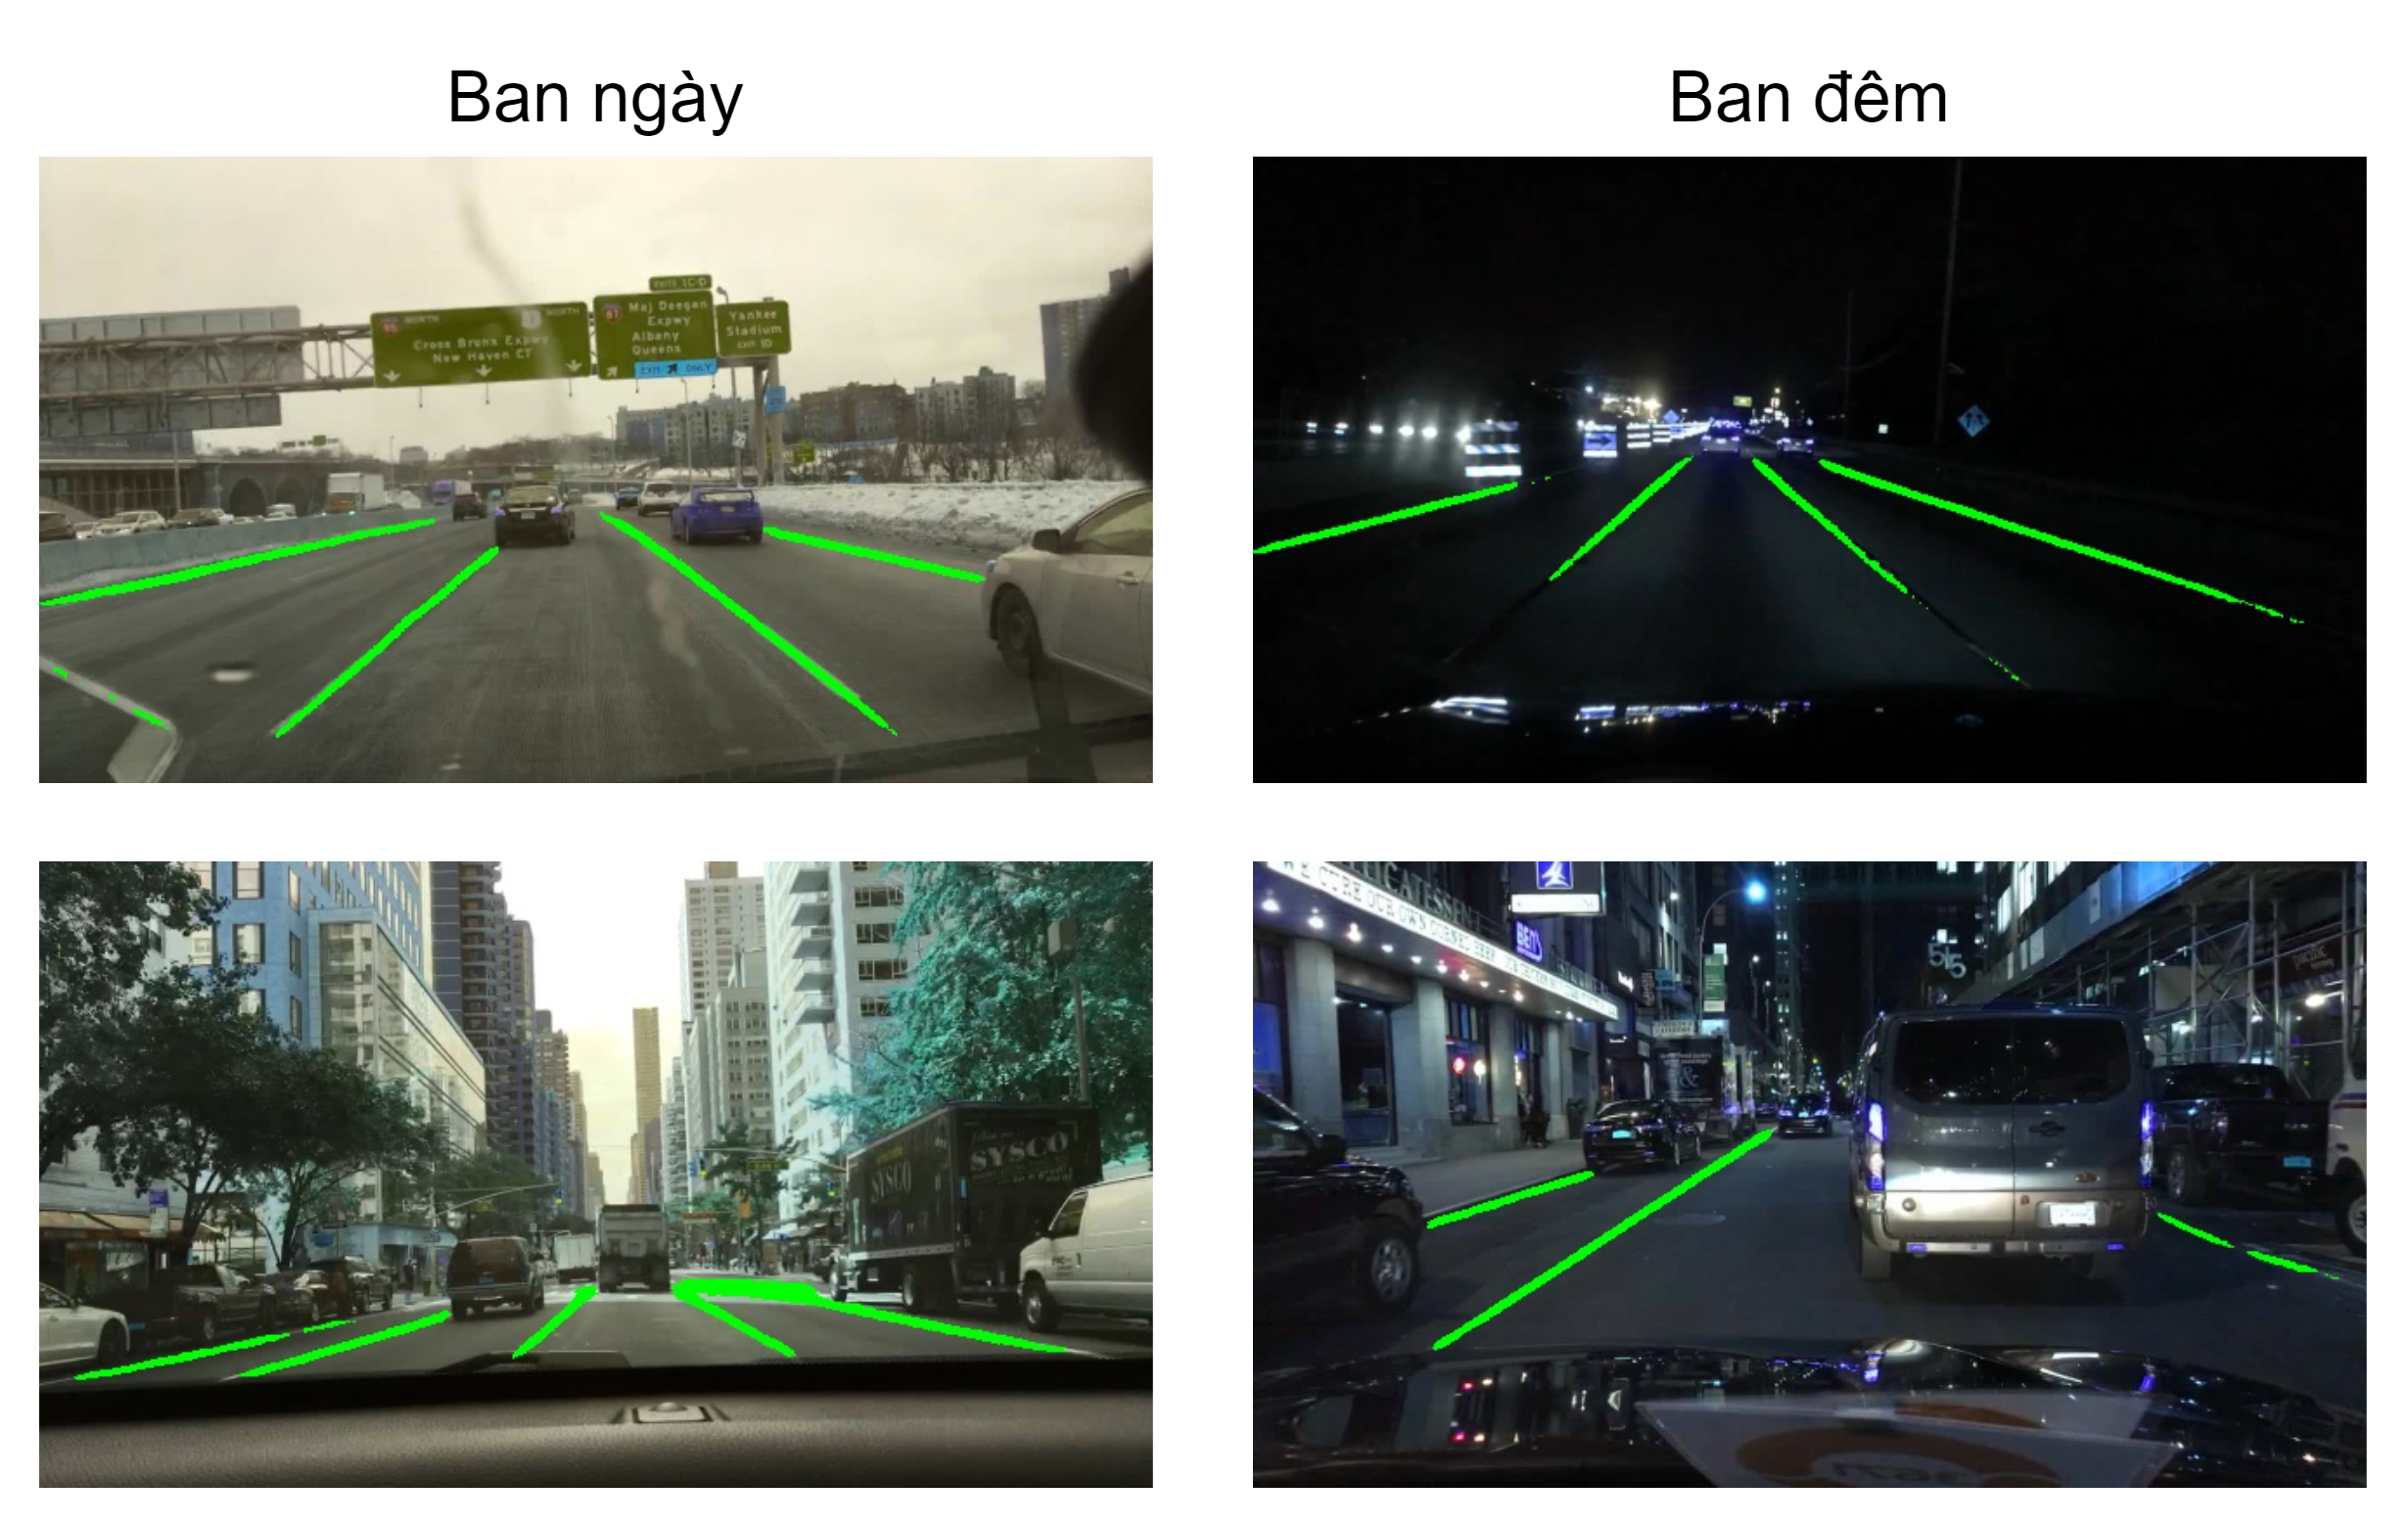
\includegraphics[width=12cm]{img/4_Implement/ai/visualization_results.png}
    \caption{\label{lane_visualization_results}Kết quả nhận diện làn đường}
\end{center}
\end{figure}\\
\subsection{Huấn luyện model}
Nhóm sử dụng model đã được train sẵn (pretrained) của tác giả, model nhận diện tốt làn đường thực tế. Tuy nhiên, vì model chỉ được huấn luyện (train) trên bộ dữ liệu thực tế nên khi nhóm thử nghiệm trên môi trường mô phỏng Gazebo\textsuperscript{\cite{gazebo}}, model đã không thể nhận diện đúng.\\
\begin{figure}[!hbt]
\begin{center}
    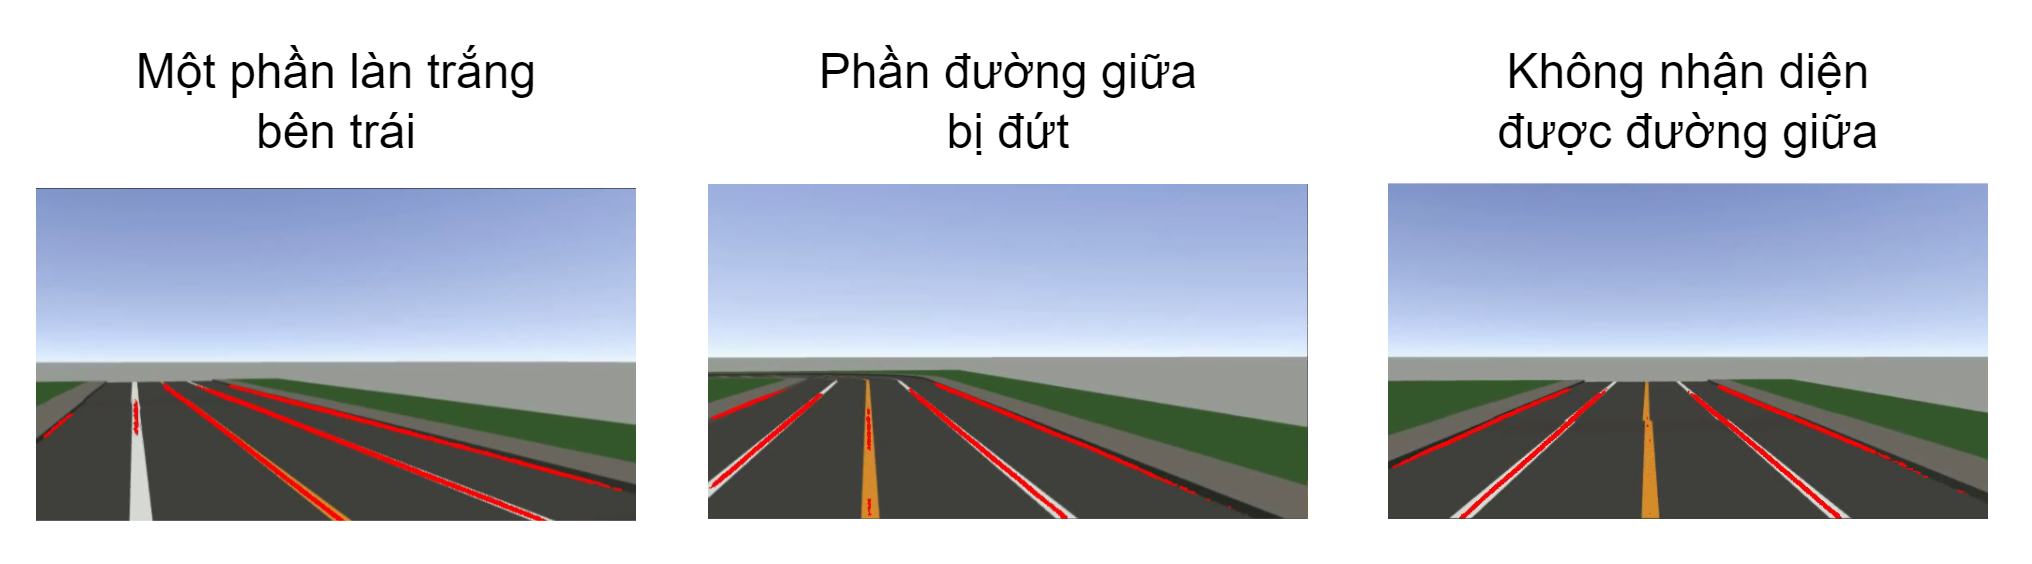
\includegraphics[width=15cm]{img/4_Implement/ai/simulation_error.png}
    \caption{Kết quả của model trước khi train thêm với data bổ sung}
\end{center}
\end{figure}\\
\textbf{Môi trường mô phỏng:}
Sau khi xác định vấn đề không thể nhận diện đúng trong môi trường mô phỏng, nhóm quyết định tiếp tục quá trình huấn luyện mô hình AI để cải thiện khả năng nhận diện của nó. Để làm điều này, nhóm đã thực hiện thu thập dữ liệu từ môi trường mô phỏng sử dụng công cụ Unity\textsuperscript{\cite{unity}}. Tổng cộng, nhóm đã thu thập 4.000 hình ảnh từ môi trường này, bao gồm các vị trí khác nhau của làn đường, vật cản, và góc độ quan sát của camera. Việc đa dạng hóa dữ liệu này giúp mô hình học được từ nhiều tình huống khác nhau, từ đó cải thiện khả năng tổng quát hóa và nhận diện trong môi trường mô phỏng. Dữ liệu thu thập từ môi trường mô phỏng sẽ được kết hợp với dữ liệu thực tế từ BDD100K\textsuperscript{\cite{bdd100k}} để tăng cường độ đa dạng và khả năng áp dụng cho cả hai môi trường thực và mô phỏng.\\\\
\textbf{Môi trường thực tế:} Với 
\noindent 
\newpage
\begin{figure}[!hbt]
\begin{center}
    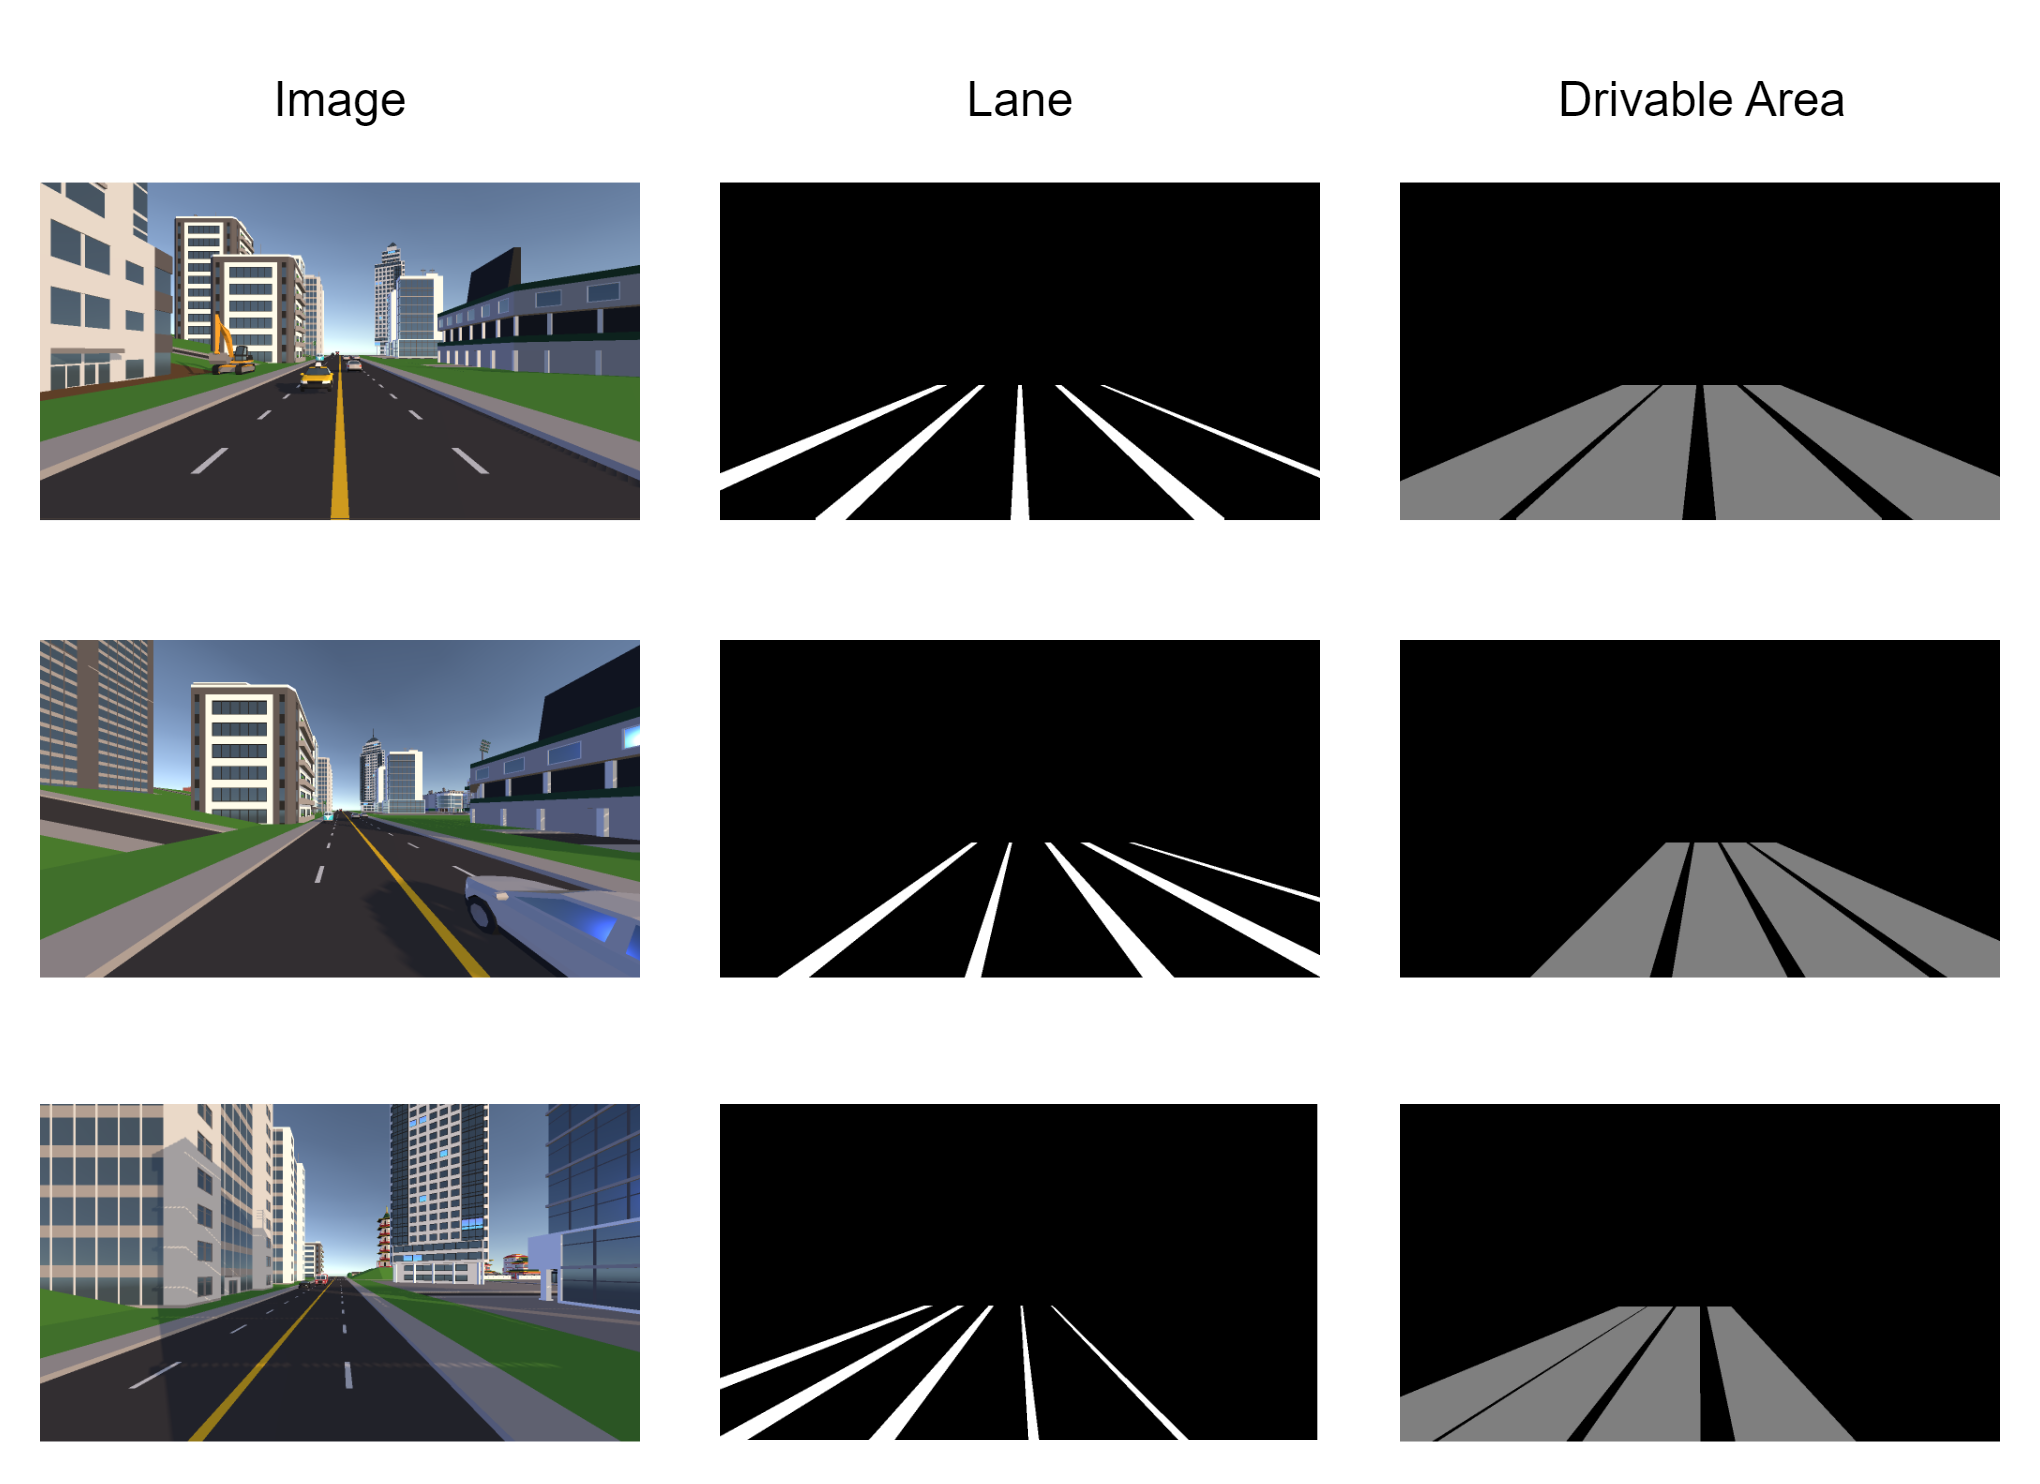
\includegraphics[width=14.5cm]{img/4_Implement/ai/simulation_data.png}
    \caption{Minh hoạ tập dữ liệu mô phỏng}
\end{center}
\end{figure}
\noindent Model sẽ được train thêm 10 epoch với batch size là 32. Qua mỗi epoch, nhóm sẽ kiểm định lại độ chính xác của model trên tập dữ liệu BDD100K. Từ đó nhóm chọn được \textbf{model\_4} (model được train thêm 4 epoch) làm model chính trong đồ án mô phỏng này
\begin{table}[!hbt]
\begin{tabular}{@{}lccccccccccc@{}}
\toprule
\textbf{Epoch}             & \textbf{0} & \textbf{1} & \textbf{2} & \textbf{3} & \textbf{4}    & \textbf{5} & \textbf{6} & \textbf{7} & \textbf{8} & \textbf{9} & \textbf{10} \\ \midrule
\textbf{Độ chính xác (\%)} & 99.0       & 99.0       & 99.0       & 98.9       & \textbf{99.0} & 98.9       & 98.5       & 98.8       & 98.3       & 98.6       & 98.4        \\
\textbf{IoU (\%)}          & 31.0       & 25.9       & 27.5       & 27.4       & \textbf{28.3} & 27.7       & 27.8       & 27.5       & 27.9       & 27.2       & 27.7        \\
\textbf{mIoU (\%)}         & 65.0       & 62.4       & 63.2       & 63.2       & \textbf{63.7} & 63.3       & 63.5       & 62.8       & 63.0       & 62.7       & 63.2        \\ \bottomrule
\end{tabular}
\caption{Thống kê đánh giá model được train thêm theo epoch}
\end{table}
\begin{figure}[!hbt]
\begin{center}
    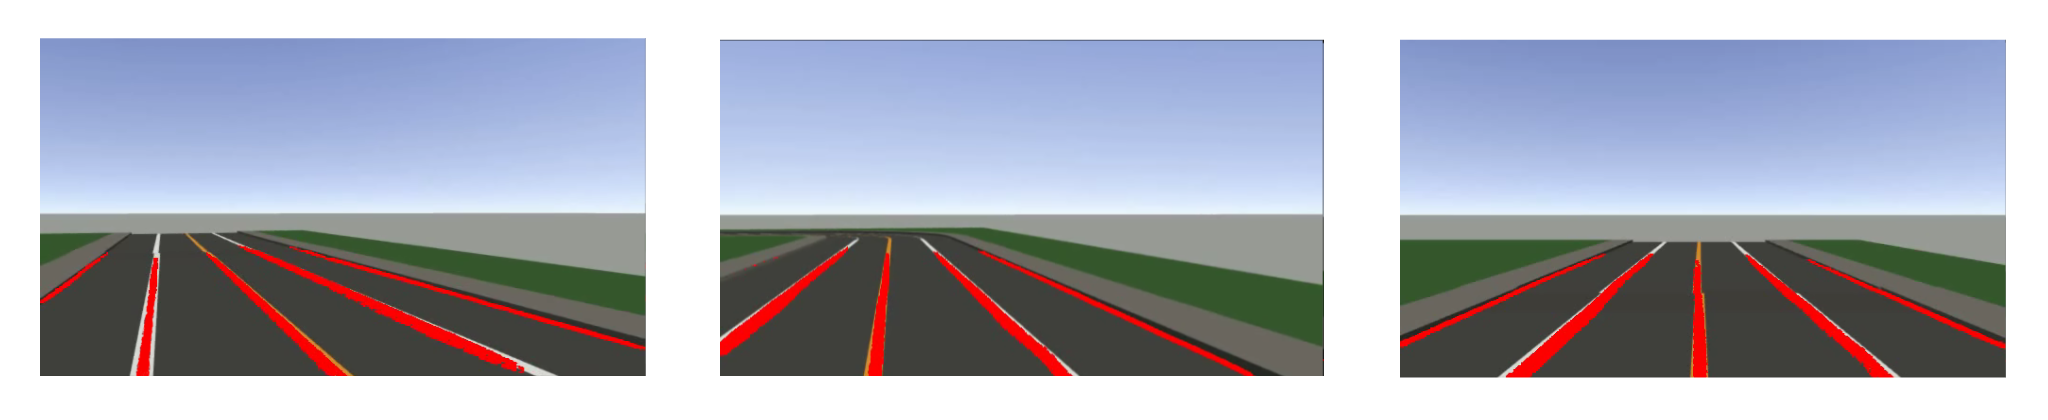
\includegraphics[width=15cm]{img/4_Implement/ai/simulation_result.png}
    \caption{Kết quả của model sau khi train thêm với data bổ sung}
\end{center}
Output hiện tại của model chỉ là ảnh RGB với hai màu trắng đen. Nhóm sẽ chuyển ảnh về dưới dạng binary để phục vụ cho quá trình phân đoạn làn đường tiếp theo. Ảnh binary là một loại hình ảnh được biểu diễn bằng các giá trị pixel chỉ có thể nhận một trong hai giá trị: 0 hoặc 1 (hoặc đen và trắng). Trong ảnh binary, mỗi pixel thường đại diện cho một phần của hình ảnh, và giá trị 0 tượng trưng cho màu đen, còn giá trị 1 tượng trưng cho màu trắng.
\end{figure}
\newpage
\subsection{Lane Fitting (Nội suy làn đường)}
Mục đích chính của module Lane Fitting là để tách các làn đường riêng biệt từ ảnh binary của model AI. Giúp ta có thể dễ dàng xác định được hình dáng, vị trí của từng làn đường.
\begin{itemize}
    \item \textbf{Input:} Kết quả nhận diện làn đường của model (dạng ảnh binary, kích thước là 640 x 360 x 1).
    \item \textbf{Output:} Trả về phương trình của tất cả làn đường 
\end{itemize}
\subsubsection{Phương pháp 1 (Hough Transform)}
\begin{figure}[h]
\begin{center}
 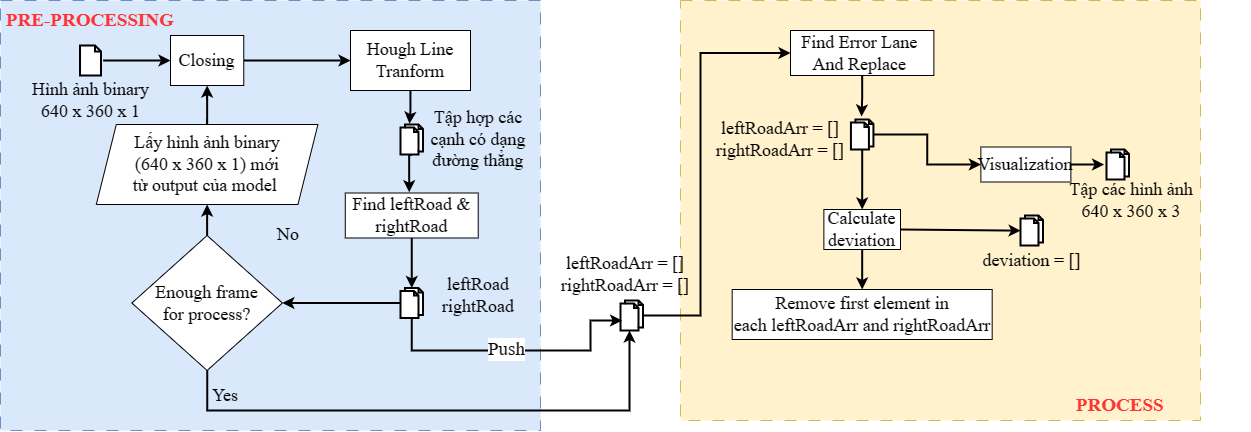
\includegraphics[width=18cm]{img/4_Implement/backend/Backend_imp.png}
 \caption{Tổng quan thuật toán của khối Backend}
 \label{back_end_cai_tien}
\end{center}
\end{figure}
\tab Dưới đây là phần giải thích chi tiết thuật toán của khối Backend sau khi được cải tiến. Khối Backend lúc này sẽ gồm 2 phần: Tiền xử lý (Pre-processing) và Xử lý (Process).\\
\tab \textbf{Pre-processing:} Khối này làm nhiệm vụ thực hiện việc tìm làn đường bên trái và làn đường bên phải của robot (không quan tâm làn đường là làn lỗi/nhiễu hay là làn đúng) cho từng ảnh (frame) trên tổng số \textbf{N} (với \textbf{N} là một ngưỡng số lượng các ảnh cần lấy để quá trình \textbf{Xử lý} đưa ra kết quả đúng nhất). Sau khi thực hiện Pre-processing trên \textbf{N} ảnh, tiến hành \textbf{Xử lý}.\\
\tab \textbf{Input:}
\begin{figure}[h]
    \centering
    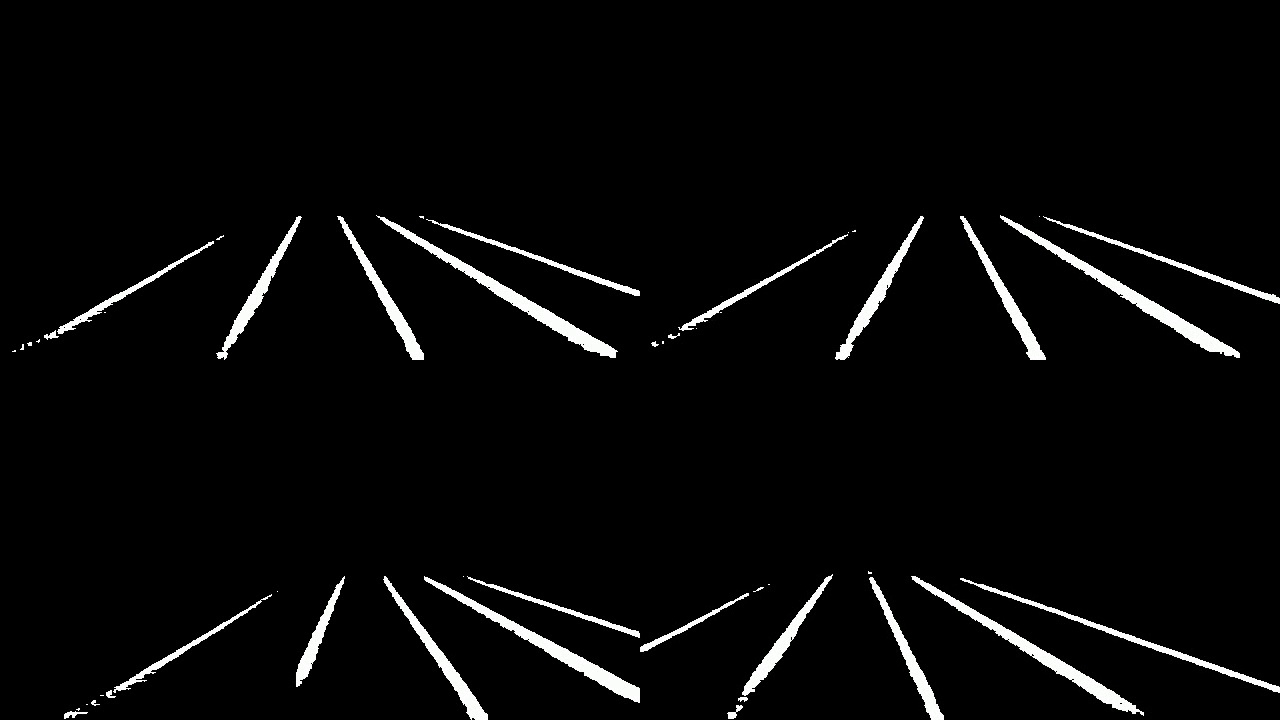
\includegraphics[width = 12cm]{img/4_Implement/backend/input.png}
    \caption{Hình ảnh minh họa cho input}
\end{figure}
\begin{enumerate}
    \item Lấy 1 ảnh mới. Tiến hành các bước 2 - 4 trên hình này.
    \item \textit{Ứng dụng Closing:} nhằm làm mịn các đường viền, đóng các lỗ nhỏ và giảm nhiễu trong ảnh.
    \begin{figure}[h]
        \centering
        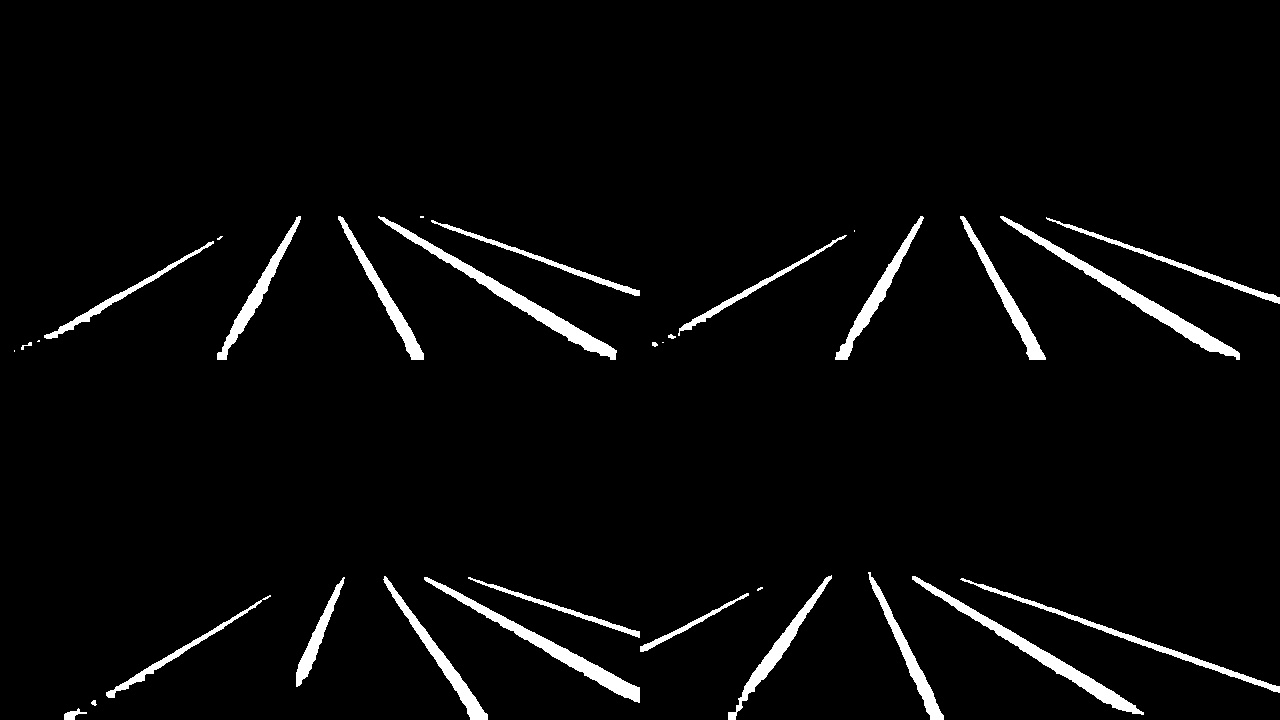
\includegraphics[width=12cm]{img/4_Implement/backend/closing.jpg}
        \caption{Hình ảnh minh họa cho làn đường sau khi ứng dụng Closing}
    \end{figure}
    \item \textit{Sử dụng thuật toán Hough Line Transform\textsuperscript{\cite{houghtransform}}:} Tìm kiếm những cạnh có dạng đường thẳng. Các đường được chia làm ba loại dựa theo góc  $\theta$ hợp giữa đường thẳng và trục hoành (Ox):
    \begin{itemize}
        \item Đường thẳng thuộc về phía bên trái có góc $\theta$ < 0.
        \item Đường thẳng thuộc về phía bên phải có góc $\theta$ > 0.
        \item Đường thẳng không thuộc về làn bên phải lẫn làn bên trái - đường nằm ngang, góc $\theta = 0$.
    \end{itemize}
    Từ tập các cạnh có dạng đường thẳng sinh ra từ thuật toán Hough Line Transform, ta thu được 2 tập đường thẳng con: 1 tập đường thẳng thuộc về làn đường phía bên trái và 1 tập đường thẳng thuộc về làn đường phía bên phải. Ta gọi tập đường thẳng thuộc phía bên trái là $L_{left} = \{ L_0, L_1,.., L_{k-1}\}$, (với $k$ là số lượng đường thẳng thỏa mãn điều kiện thuộc về làn đường phía bên trái) và tập đường thẳng thuộc phía bên phải là $L_{right} = \{L_0, L_1,.., L_{m-1}\}$ (với $m$ là số lượng đường thẳng thỏa mãn điều kiện thuộc về làn đường phía bên phải).
    \begin{figure}[h]
        \centering
        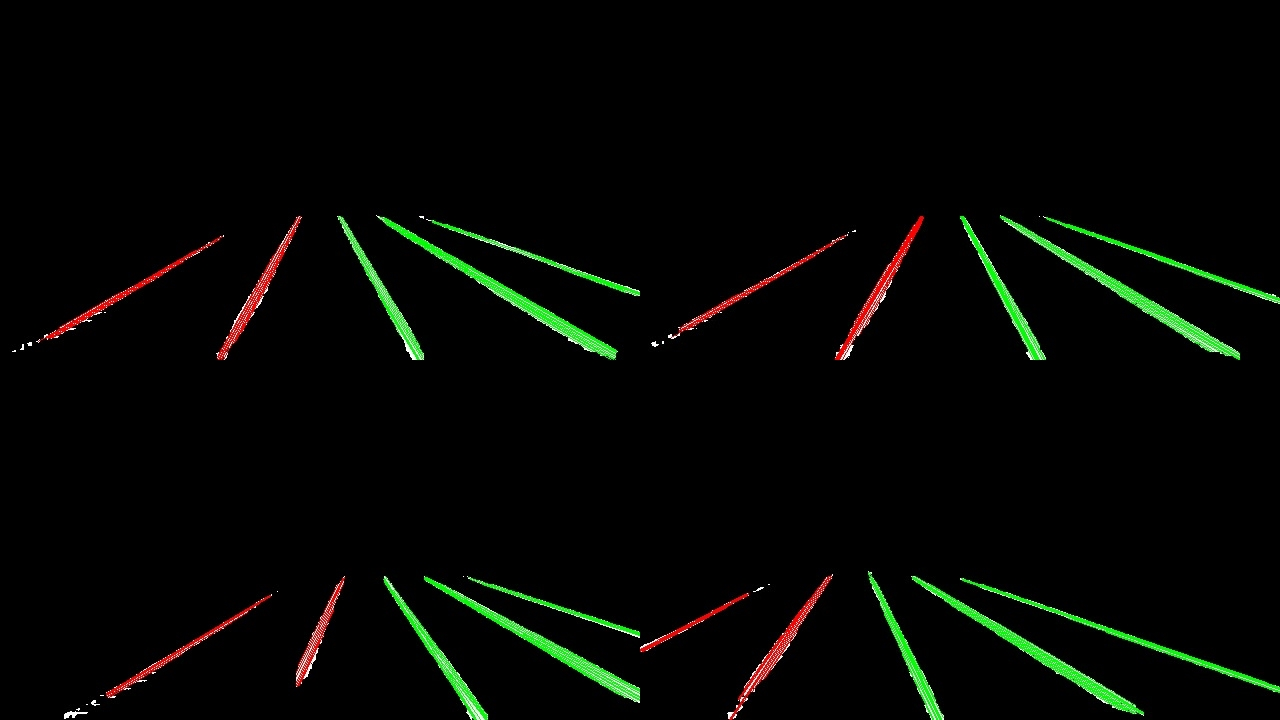
\includegraphics[width=12cm]{img/4_Implement/backend/hough_line.jpg}
        \caption{Hình ảnh minh họa làn đường sau khi ứng dụng Hough Line Transform}
    \end{figure}
    \item \textit{Find leftRoad và rightRoad}: Xác định 01 làn đường trái và 01 làn đường phải của robot. Cách xác định như sau:
    \begin{itemize}
        \item Tìm trong tập $L_{left}$ 01 đường thẳng sao cho trị tuyệt đối của góc $\theta$ hợp bởi đường thẳng này và trục hoành có giá trị lớn nhất. Ta nhận đường thẳng này là làn đường phía bên trái của robot. Gọi đường thẳng này là leftRoad. Trong trường hợp không tìm thấy đường thẳng (do mất toàn bộ làn đường bên trái), leftRoad lúc này không tồn tại.
        \item Tìm trong tập $L_{right}$ 01 đường thẳng sao cho  góc $\theta$ hợp bởi đường thẳng này và trục hoành có giá trị lớn nhất. Ta nhận đường thẳng này là làn đường phía bên phải của robot. Ta gọi đường thẳng này là rightRoad. Trong trường hợp không tìm thấy đường thẳng (do mất toàn bộ làn đường bên phải), rightRoad lúc này không tồn tại.
    \end{itemize}
    Lúc này, ta được leftRoad và rightRoad lần lượt là đường thẳng thuộc làn đường bên trái và đường thẳng thuộc làn đường bên phải của robot, kết quả này có thể bao gồm cả đường thẳng thuộc trường hợp nhiễu hoặc không tồn tại. Ta thêm leftRoad vào tập các làn đường bên trái và rightRoad vào tập các làn đường bên phải nhằm phục vụ cho các bước xử lý tiếp theo. Nếu chưa đủ \textit{N} frame, quay lại bước 1. Nếu đã đủ, qua bước \textbf{Xử lý}.    
\end{enumerate}
\tab \textbf{Xử lý:} Nhiệm vụ của bước này là lọc ra những đường thẳng lỗi và thay thế chúng (nếu có). Chi tiết bước này trình bày như sau:
\begin{enumerate}
    \item \textit{Find error line and replace:} Ta tiến hành tìm kiếm và thay thế những đường thẳng lỗi cho làn đường bên trái và làn đường bên phải như sau:

    
    \begin{itemize}
        \item Gọi $\theta_{n}^{l}$ là trị tuyệt đối của góc hợp bởi đường thẳng bất kì thuộc tập làn đường bên trái (thu được từ bước \textbf{Xử lý} trước đó) với trục hoành. 
        \item Gọi $\theta_{n}^{r}$ là góc hợp bởi đường thẳng bất kì thuộc tập làn đường bên phải trước đó (thu được từ bước \textbf{Xử lý} trước đó) với trục hoành .
        % \item $\theta_{l} = [|\theta_{0}^{l} - \theta_{n}^{l}|, |\theta_{1}^{l} - \theta_{n}^{l}|,...|\theta_{k-1}^{l} - \theta_{n}^{l}|]$. Với k là số lượng đường thẳng có trong tập làn đường bên trái đang xử lý, k $\leq$ \textit{num}.
        % \item $\theta_{r} = [|\theta_{0}^{r} - \theta_{n}^{r}|, |\theta_{1}^{r} - \theta_{n}^{r}|,...|\theta_{m-1}^{r} - \theta_{n}^{r}|]$. Với m là số lượng đường thẳng có trong mảng làn đường bên phải đang xử lý, m $\leq$ \textit{num}.
        \item Gọi $\theta_{i}^{l}$ là góc hợp bởi đường thẳng thứ $i$ ($i = \{0,1,...,N-1\}$) thuộc tập làn đường bên trái với trục hoành.
        \item Gọi $\theta_{i}^{r}$ là góc hợp bởi đường thẳng thứ $i$ ($i = \{0,1,...,N-1\}$) thuộc tập làn đường bên phải với trục hoành.
        \item Gọi $\gamma$ là ngưỡng chấp nhận được. Cụ thể hơn: $|\theta_{i}^{l} - \theta_{n}^{l}| < \gamma$ và $|\theta_{i}^{r} - \theta_{n}^{r}| < \gamma$, với $i = \{0,1,...,N-1\}$. Những đường thẳng có trị tuyệt đối của hiệu lớn hơn sẽ được xem là những đường thẳng lỗi, và sẽ được thay thế bằng đường thẳng đứng trước nó (trong tập). Tuy nhiên, với những trường hợp không thể tính góc $\theta$ do đường thẳng không tồn tại, chương trình sẽ trả về "Không nhận diện được".
    \end{itemize}
    Kết quả cuối cùng của bước này, ta thu được tập các làn đường bên trái $L_{l} = \{ L_0, L_1,.., L_{k-1}\}$ và tập các làn đường bên phải $L_{r} = \{L_0, L_1,.., L_{k-1}\}$, $k \leq N$ chỉ bao gồm những làn đường đúng.
    \item \textit{Calculate deviation:} Từ tập các đường thẳng bên trái và mảng các làn đường bên phải, ta lấy ra leftRoad thứ $i$ và rightRoad thứ $i$, $i = \{0,1,...,N-1\}$, ta có thể tính được độ lệch của robot so với tâm làn đường thứ i như sau:
    \begin{itemize}
        \item Tìm giao điểm của leftRoad với trục hoành. Gọi điểm này là $it_{l}$.
        \item Tìm giao điểm của rightRoad với trục hoành. Gọi điểm này là $it_{r}$.
        \item Tìm phương trình đường thẳng của làn đường trung tâm: Là đường thẳng nối 2 điểm: giao điểm của leftRoad và rightRoad với trung điểm của $it_{l}$ và $it_{r}$
        \item Tính độ dài hình chiếu của đường thẳng này xuống trục hoành. Độ dài của hình chiếu chính là độ lệch $d$ chúng ta cần tìm.
    \end{itemize}
    Kết quả của bước này là mảng các giá trị \textit{d} tương ứng với các frame.
    \item \textit{Visualization:} Từ tập các đường thẳng bên trái và tập các làn đường bên phải, ta lấy ra leftRoad thứ $i$ và rightRoad thứ $i$, $(0 \leq i \leq k-1)$, $k \leq N$, ta có thể visualize kết quả nhận diện làn đường trái và làn đường phải của khối Backend cải tiến lên ảnh thứ i tương ứng. Kết quả như hình \ref{final_result_of_BE}.
    \begin{figure}[h]
        \centering
        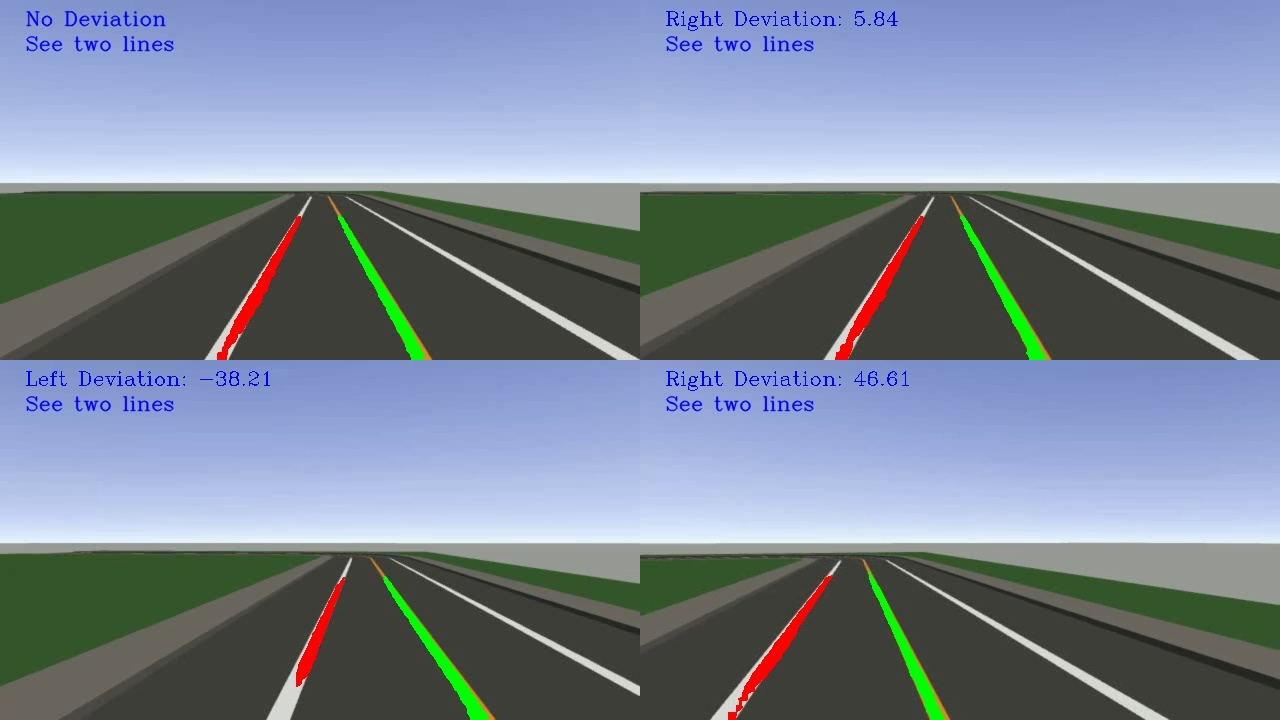
\includegraphics[width=12cm]{img/4_Implement/backend/ressult.jpg}
        \caption{Hình ảnh kết quả cuối cùng của khối Backend}
        \label{final_result_of_BE}
    \end{figure}
    \item Xóa phần tử đầu tiên của mảng làn đường bên trái và mảng làn đường bên phải.
\end{enumerate}
\textbf{Ưu điểm và nhược điểm}
\subsubsection{Phương pháp 2 (K–means Clustering)}
\textbf{Ưu điểm và nhược điểm}
\subsubsection{Phương pháp 3 (Sliding Window)}
Bởi vì số cluster không thể xác định do các cụm làn đường luôn luôn thay đổi. Do đó, nhóm đã chuyển sang sử dụng phương pháp sliding window. Với sliding window, ta có thể linh hoạt xác định các vùng có khả năng chứa làn đường trên ảnh.\\\\
\textbf{Perspective Transform:}\
Trước khi áp dụng sliding window, ta cần thực hiện biến đổi \textbf{camera view} sang \textbf{bird’s eye view}, giúp thuận tiện cho việc phân đoạn và xác định làn đường. Khi nói về Affine Transformations, chúng ta nói đến một loại phép biến đổi hình học trong không gian hai hoặc ba chiều. Khi áp dụng phép biến đổi này, các điểm trong không gian được di chuyển, xoay và co giãn để tạo thành một hình học mới. Điều này có thể được biểu diễn bằng ma trận biến đổi affine.\\\\
Ma trận biến đổi Affine được biểu diễn dưới dạng ma trận $3x3$ cho biến đổi trong
không gian hai chiều. Ma trận này bao gồm các thông số để biểu diễn các phép biến đổi
như dịch chuyển, xoay và co giãn. Cụ thể, ma trận Affine cho phép dịch chuyển bằng
cách thêm một vector tịnh tiến vào tọa độ ban đầu của điểm. Xoay được thực hiện bằng
cách sử dụng các phép toán ma trận để xoay điểm quanh một trung tâm quay. Co giãn
được thực hiện bằng cách thực hiện phép nhân ma trận với một vector giữa các hệ số co
giãn tương ứng cho mỗi chiều.\\\\
Những vị trí này sẽ tương ứng với những vị trí xác định trong bề mặt bird’s eye view. Vậy nhóm sẽ có bốn cặp điểm ở bề mặt thực tế tương ứng với bề mặt bird’s eye view. Nhóm sử dụng hàm \textbf{cv2.getPerspectiveTransform} để suy ra được ma trận biến đổi affine từ bốn cặp điểm trên. Ma trận này đặc trưng cho vị trí của camera so với robot và bề mặt nằm ngang, do đó các thay đổi như thay đổi về chiều cao robot hoặc vị trí camera, nhóm sẽ phải thực hiện lại bước thiết lập các điểm để đảm bảo tính đúng đắn của ma trận affine.
\newpage
\begin{figure}[!hbt]
\begin{center}
    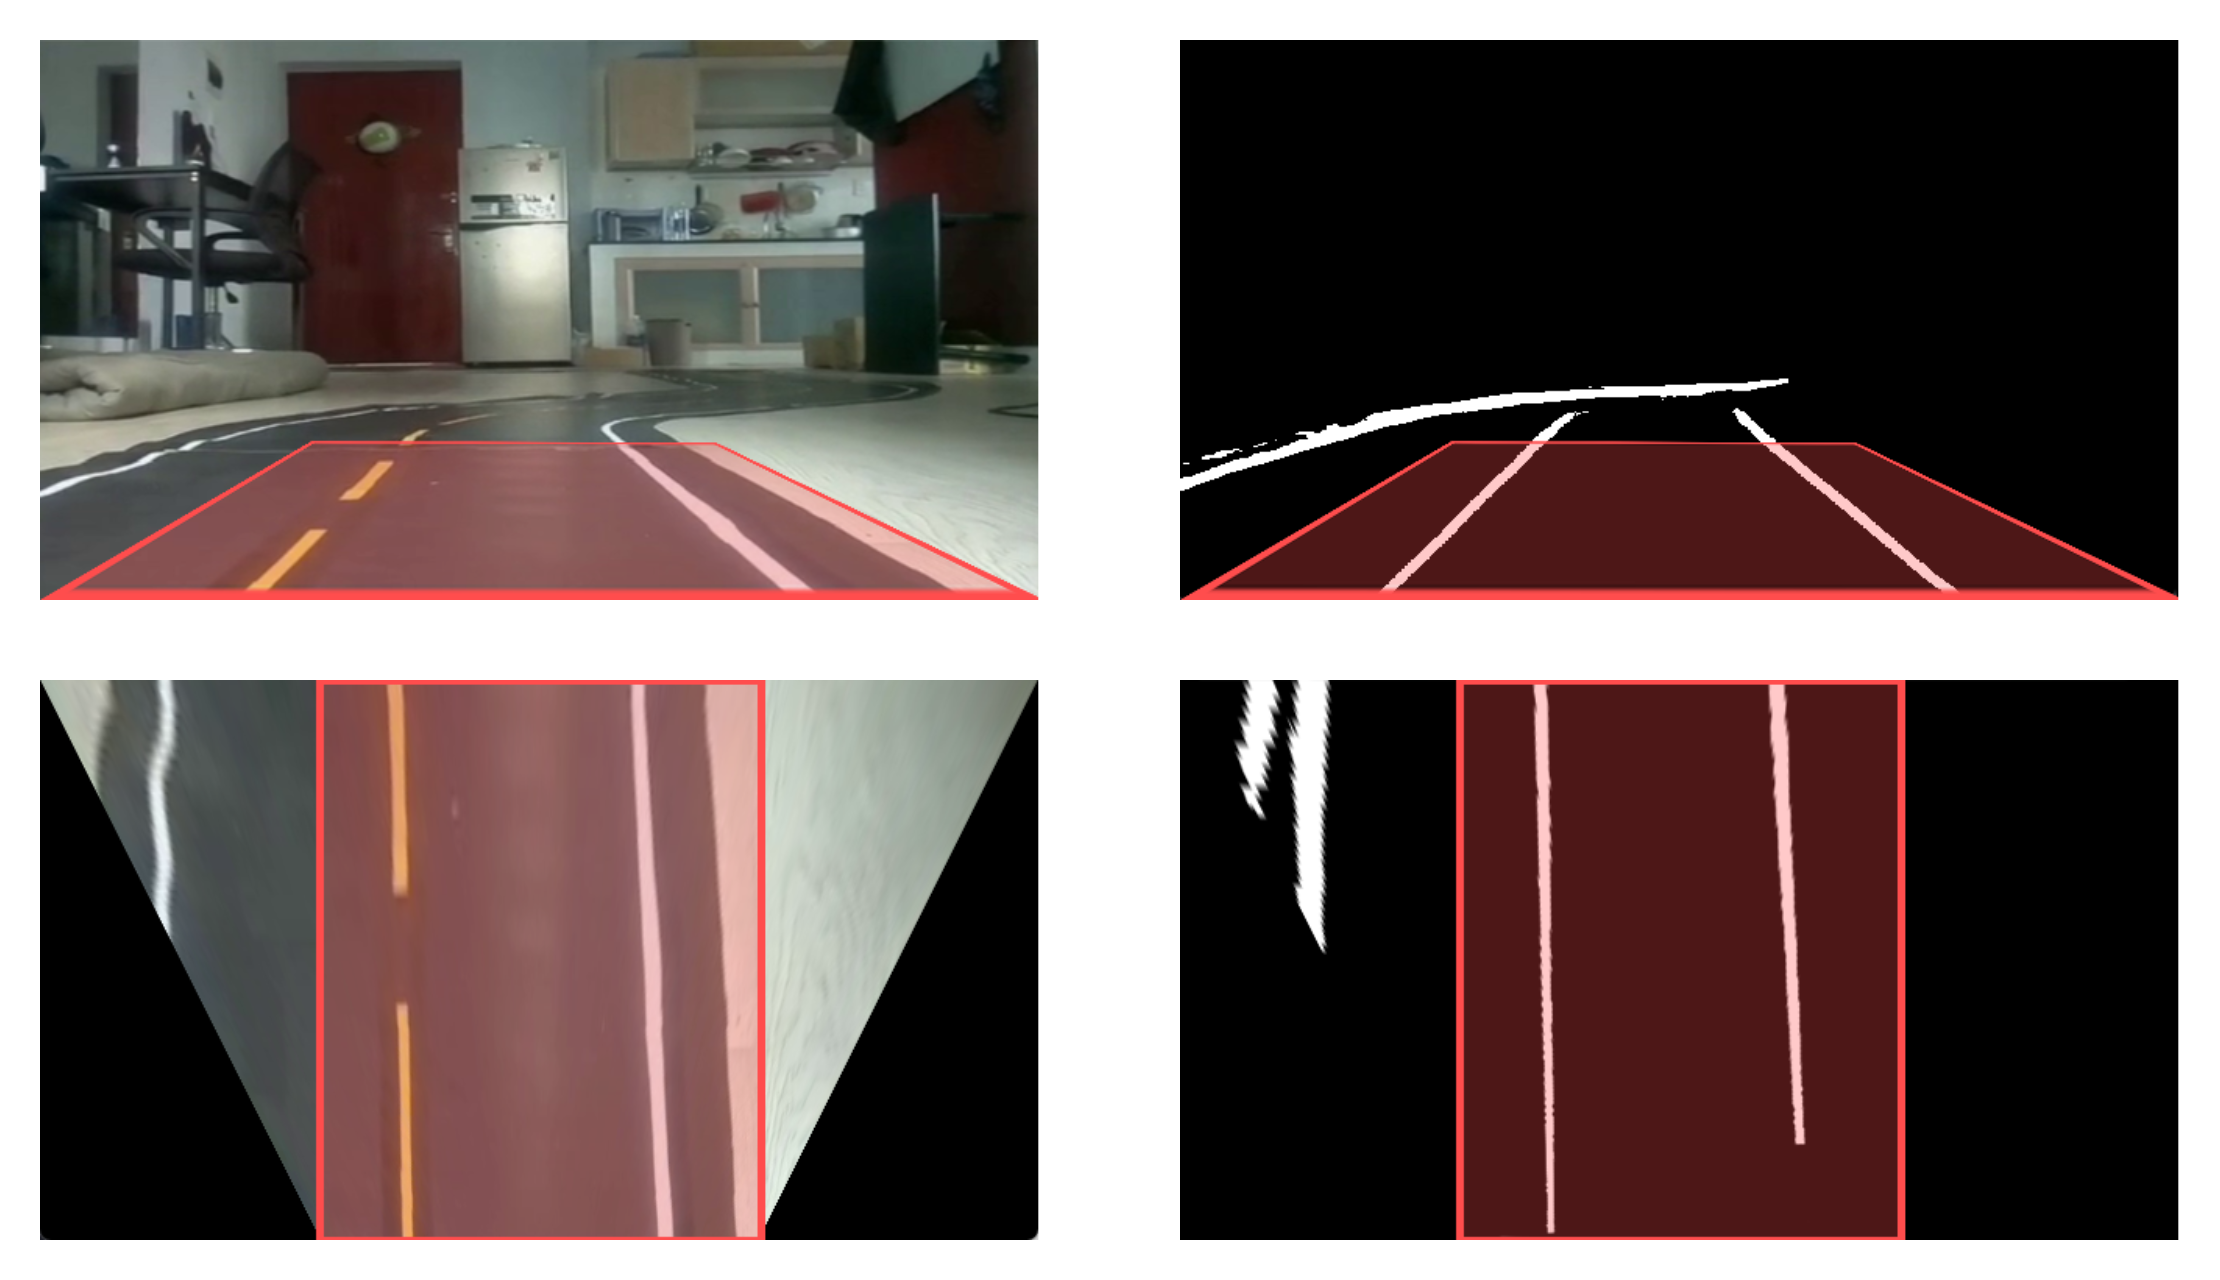
\includegraphics[width=15cm]{img/4_Implement/sliding_window/perspective_transform.png}
    \caption{Ảnh từ camera view và bird's eye view}
\end{center}
\end{figure}
\noindent Vị trí bốn điểm ở hệ toạ độ camera: $\begin{bmatrix}190 & 250\\460 & 250\\640 & 360\\0 & 360\end{bmatrix}$\\
Vị trí bốn điểm ở hệ toạ độ thực: $\begin{bmatrix}180 & 100\\460 & 100\\460 & 360\\180 & 360\end{bmatrix}$\\
Ma trận affine thu được: $M = \begin{bmatrix}-0.5 & -1.9 & 484.97\\-5.33 & -3.24 & 762.42\\-1.43 & -0.005 & 1.0\\\end{bmatrix}$\\
Khi đã có ma trận affine, Ta chuyển một điểm từ hệ toạ độ camera ($x_1$, $y_1$) sang hệ toạ độ
bird eye's view ($x_2$, $y_2$) như sau:
\begin{equation}
    \begin{bmatrix}x_2\\y_2\\1\end{bmatrix} = \begin{bmatrix}x_1\\y_1\\1\end{bmatrix}M
\end{equation}
Ta có $M_{inv}$ là ma trận đảo ngược của $M$ để biến đổi dữ liệu từ hệ toạ độ bird eye's view về hệ toạ độ camera, thuận tiện cho việc visualize kết quả \\\\
\textbf{Sliding Window:}
Dưới đáy của ảnh binary, một sliding window có chiều rộng bằng chiều rộng của ảnh sẽ di chuyển từ dưới lên trên cho đến khi tìm thấy cụm pixel đầu tiên của làn đường. Cụm pixel đầu tiên này được xác định là điểm bắt đầu của một làn đường. Từ cụm pixel này, một sliding window thứ hai được sử dụng để trích xuất tất cả các pixel thuộc về làn đường đó. Mặc dù chiều cao của cửa sổ này giống như cửa sổ trước, tuy nhiên, chiều rộng sẽ lớn hơn một chút so với chiều rộng của cụm pixel đầu tiên. Sau khi sliding window thứ hai đã được áp dụng, các cụm pixel của làn đường đó sẽ được loại bỏ khỏi ảnh. Quá trình này sẽ được lặp lại cho đến khi tất cả các làn đường đã được trích xuất hoàn toàn.\\
\begin{figure}[!hbt]
\begin{center}
    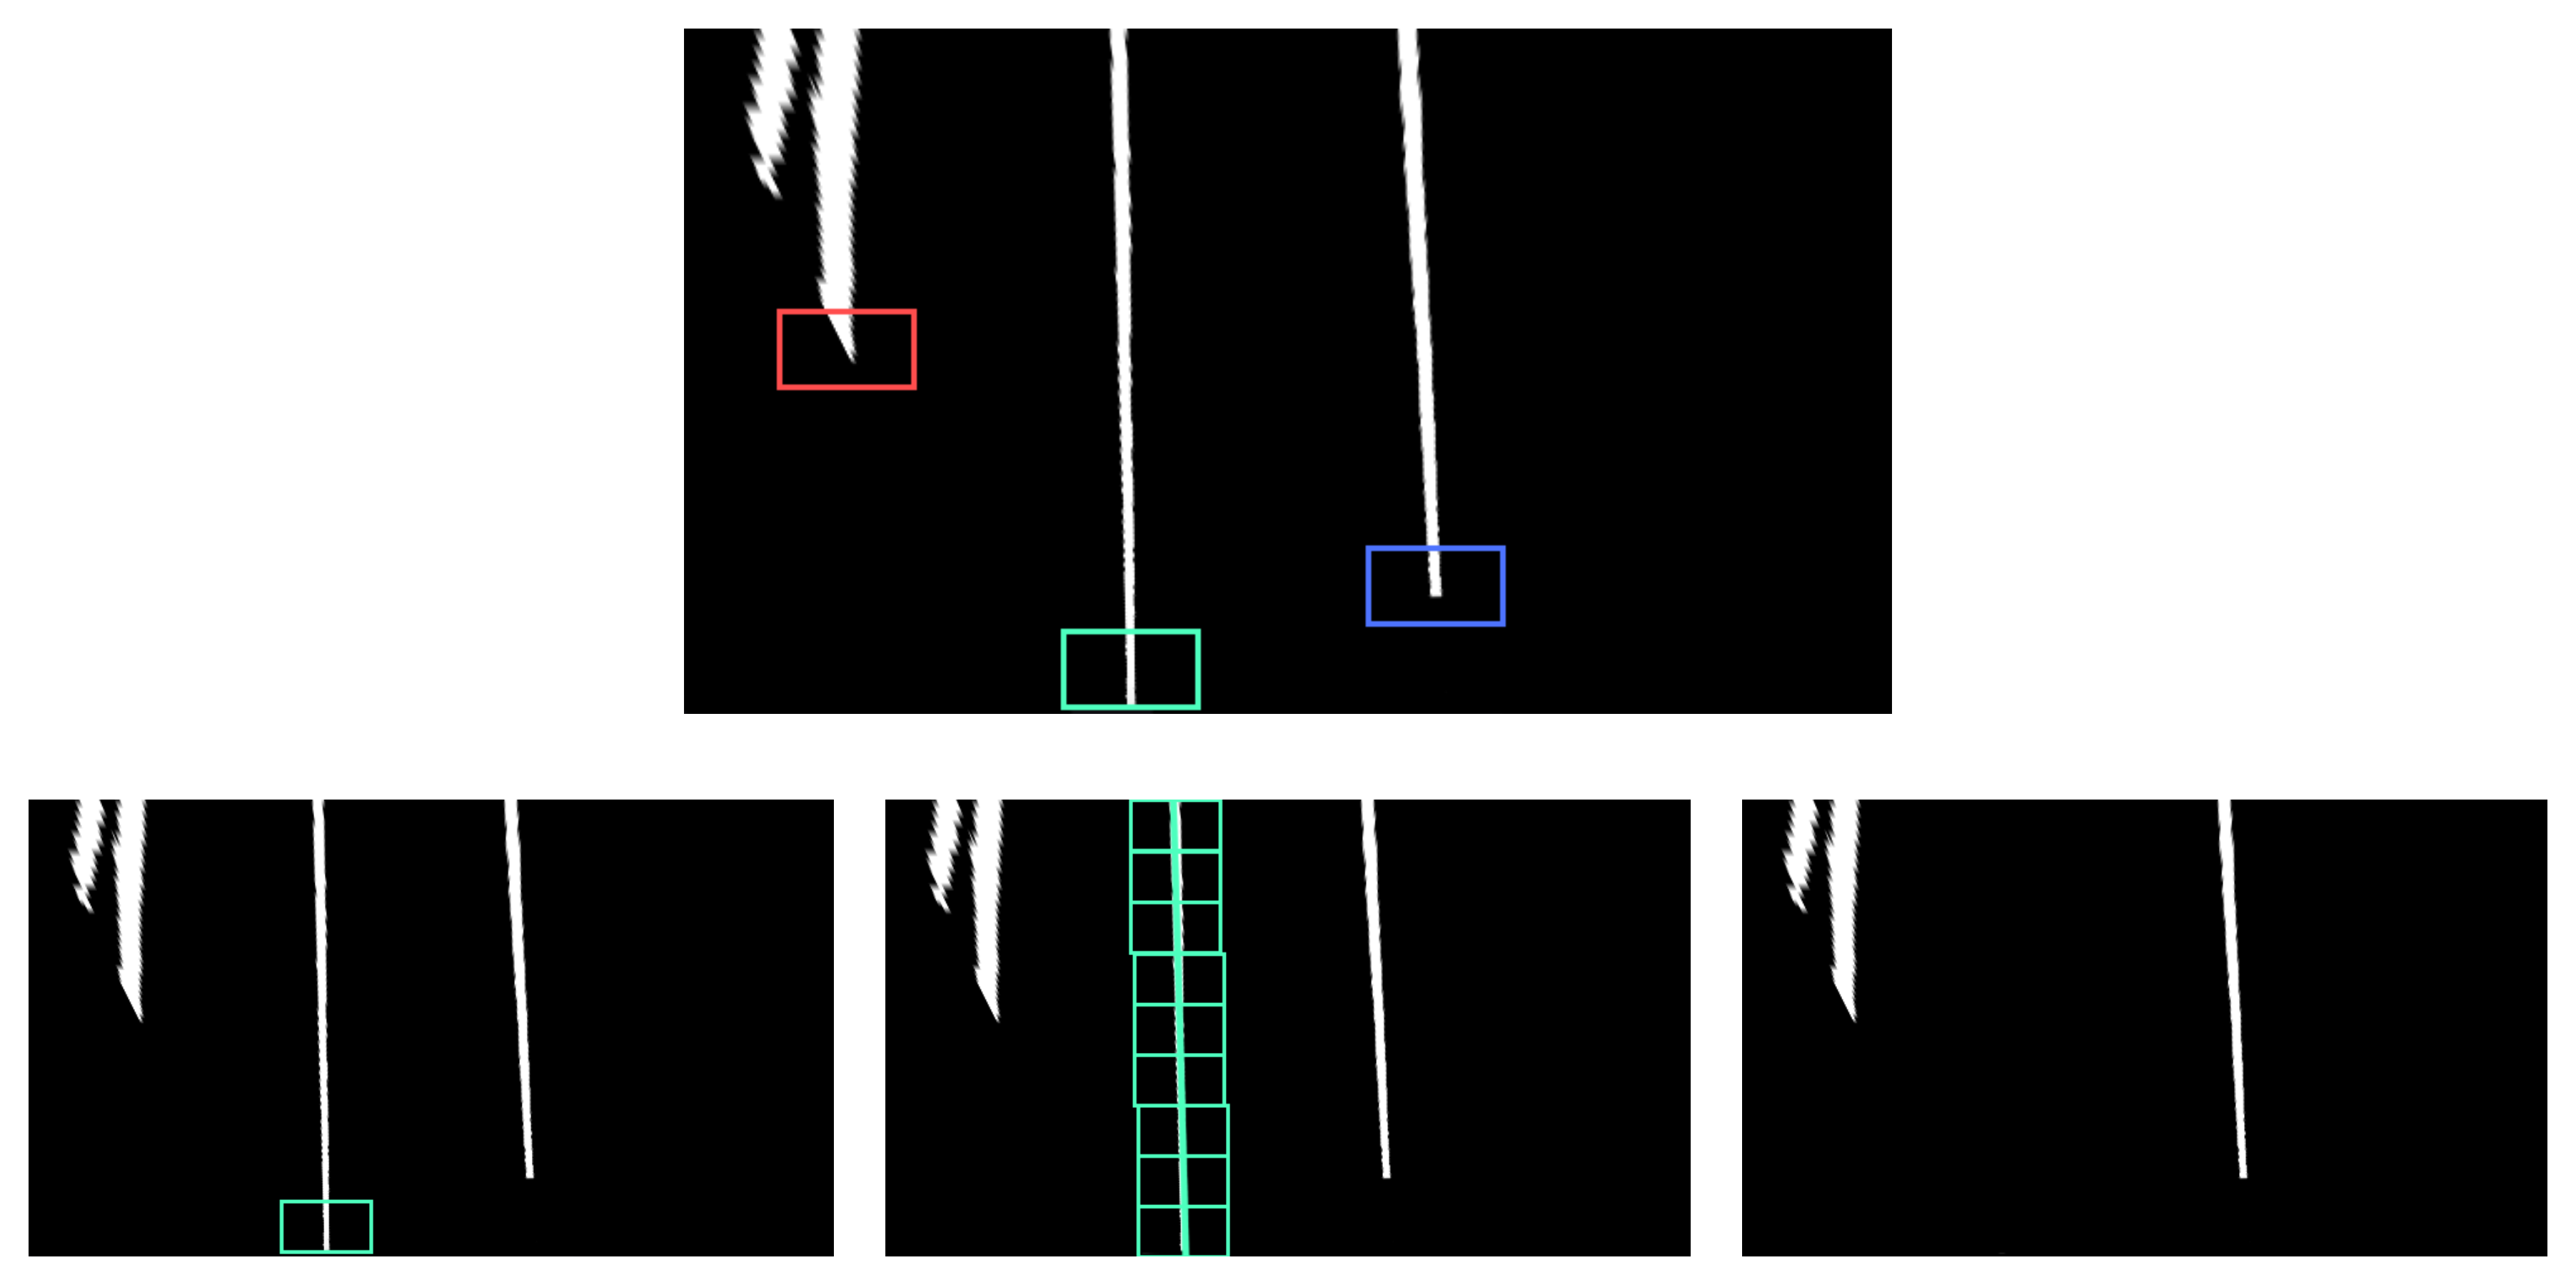
\includegraphics[width=15cm]{img/4_Implement/sliding_window/fitting.png}
    \caption{(a) Sliding window thứ nhất tìm cụm pixel đầu tiên; (b) Sliding widow thứ hai bắt đầu tại cụm pixel đầu tiên; (c) Sliding window tìm tất cả cụm pixel làn đường; (d) Xoá các cụm pixel của làn đường và lặp lại bước a}
\end{center}
\end{figure}\\
Nhóm đã cải tiến thêm thuật toán để bỏ qua việc trích xuất làn đường trong các trường hợp sau:
\begin{itemize}
    \item Làn đường trích xuất có độ dài ngắn
    \item Hai làn đường kế tiếp nhau có khoảng cách quá nhỏ so với độ rộng của robot
    \item Thiết lập ngưỡng tối đa làn đường có thể trích xuất
\end{itemize}
Các cải tiến này giúp tăng cường hiệu suất và độ chính xác của thuật toán, đồng thời giảm thiểu các trường hợp sai sót và tối ưu hóa quá trình trích xuất làn đường\\\\
\textbf{Curve Fitting:}
Sau khi một làn đường được trích xuất, ta có thể dễ dàng dùng hồi quy tuyến tính để nội suy làn đường. Phương trình làn đường sẽ có dạng như sau:
\begin{equation}
    x = ay^2 + by + c
\end{equation}
\begin{figure}[!hbt]
    \begin{subfigure}{0.5\textwidth}
        \centering
        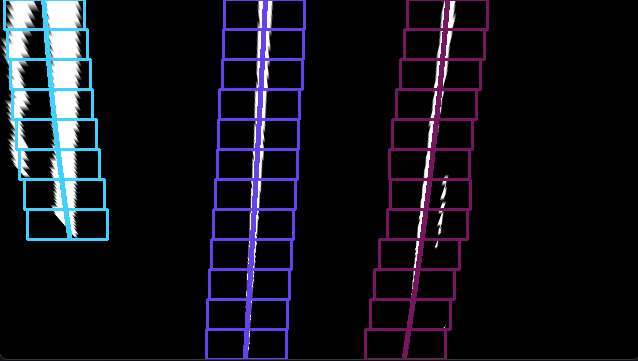
\includegraphics[width=7.5cm]{img/4_Implement/sliding_window/straight.png}
        \caption{Làn đường thẳng}
    \end{subfigure}%
    \begin{subfigure}{0.5\textwidth}
        \centering
        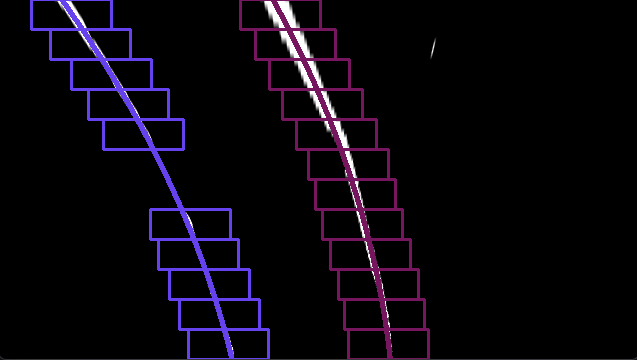
\includegraphics[width=7.5cm]{img/4_Implement/sliding_window/curve.png}
        \caption{Làn đường cong}
    \end{subfigure}
    \caption{Minh hoạ Curve Fitting trên làn đường}
\end{figure}\\
\textbf{Ưu điểm và nhược điểm}
\subsubsection{Phân tích, tổng hợp các phương pháp}
\newpage
\subsection{Lane Tracking}
\begin{itemize}
    \item \textbf{Input:} Phương trình các làn đường
    \item \textbf{Output:} Độ lệch của robot
\end{itemize}
\subsubsection{Xác định làn đường trái, phải}
Sau khi có tập hợp các đường thẳng, ta sẽ sắp xếp chúng theo độ lệch và xác định làn trái và phải gần nhất với robot. Độ lệch của làn đường sẽ được tính bằng tổng của toạ độ x của mỗi điểm trên làn đường và chia cho chiều cao của ảnh:
\begin{equation}
    d = \frac{w}{2} - \frac{\sum_{y = 0}^{h}x(y)}{h}
\end{equation}
Trong đó,
\begin{itemize}
    \item w, h: Kích thước của ảnh
    \item x = x(y), y: Toạ độ của một điểm trên phương trình làn đường
    \item d: Làn đường sẽ nằm bên trái nếu độ lệch nhỏ hơn 0 và ngược lại, làn đường sẽ nằm bên phải
\end{itemize}
\begin{figure}[!hbt]
\begin{center}
    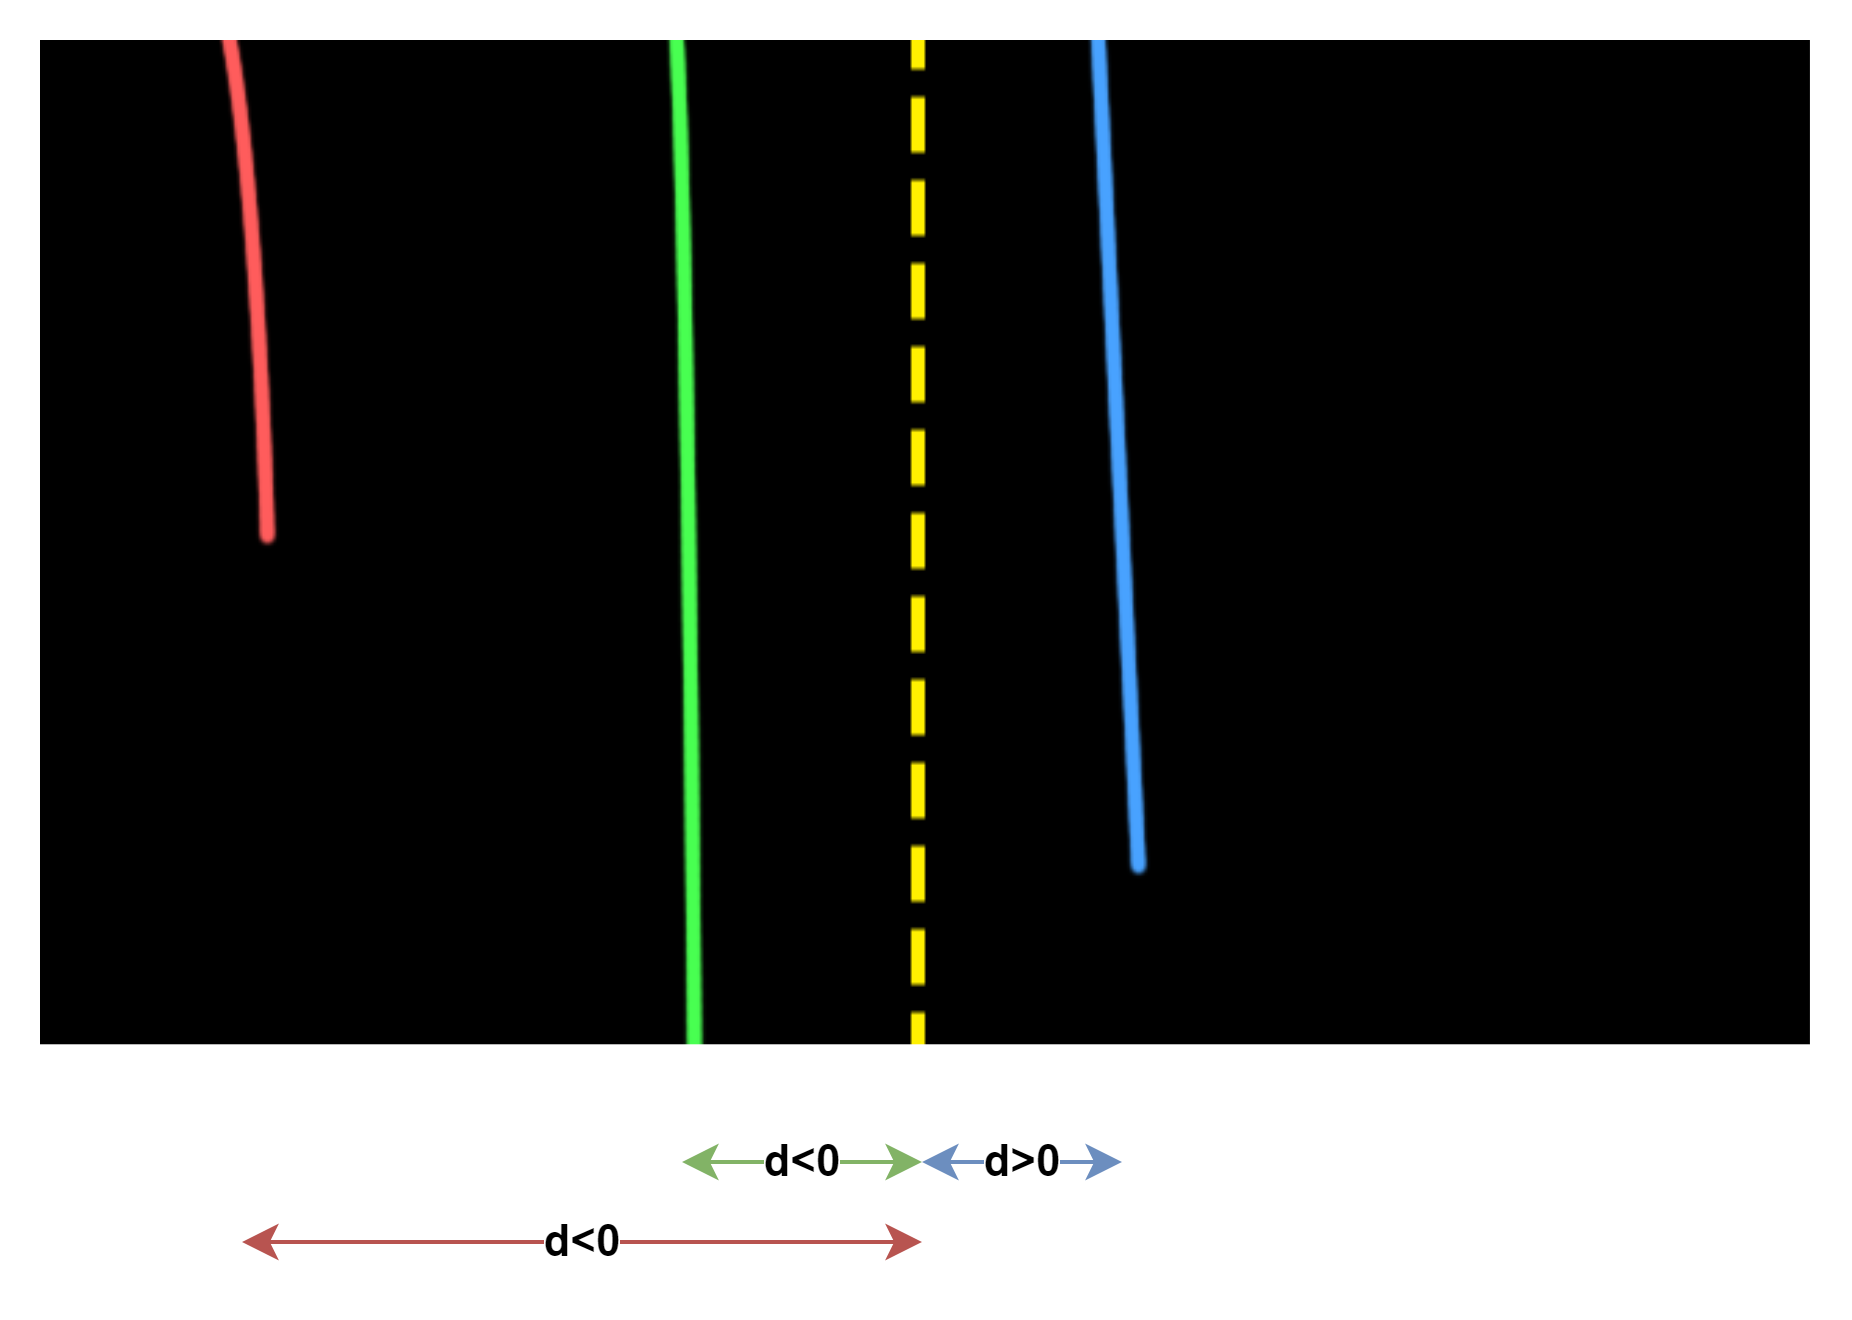
\includegraphics[width=13cm]{img/4_Implement/lane_tracking/lane_distance.png}
    \caption{Minh hoạ độ lệch các làn đường}
\end{center}
\end{figure}
\subsubsection{Nội suy làn đường giữa dựa trên dữ kiện làn đường trái, phải}
Để tìm được độ lệch của robot thì ta chỉ cần xác định được làn đường giữa và độ lệch robot chính là độ lệch của làn đường giữa. Dựa vào dữ kiện hai làn đường trước đó, ta sẽ nội suy được làn đường giữa trong các trường hợp sau:\\\\
\textbf{Có đủ dữ kiện cả 2 làn:} Phương trình làn đường giữa sẽ được tính bằng:
\begin{equation}
    x = \frac{a_L + a_R}{2}y^2 + \frac{b_L + b_R}{2}y + \frac{c_L + c_R}{2}
\end{equation}
Trong đó,
\begin{itemize}
    \item $a_L, b_L, c_L$: Hệ số phương trình làn đường trái
    \item $a_R, b_R, c_R$: Hệ số phương trình làn đường phải
\end{itemize}
\textbf{Chỉ có dữ kiện của 1 làn}: Bởi vì việc phân đoạn làn đường của mô hình AI có diễn ra sai sót, hoặc không đủ mạnh để có thể có được hoàn toàn hai làn đường, mà chỉ phát hiện được một làn đường (do có vật thể chắn, hoặc góc xoay camera dẫn đến khuất mạnh phần đường còn lại, ...). Việc dựa trên làn đường ở frame trước sẽ dẫn đến sai sót khi view camera thay đổi nhiều. Để xác định làn đường còn lại, nhóm sử dụng dữ kiện từ một làn đường hiện tại và ánh xạ song song với khoảng cách giữa hai làn đường đã biết. Cụ thể:
\begin{itemize}
    \item Cho một làn đường biết trước $L = L_i$ với $i \in \{L, R\}$
    \item Cho $d$ là khoảng cách giữa hai làn đường đã biết trước
    \item $\beta$ là làn đường cần tìm, $\beta \in \{L_L, L_R\}$. Nếu ta đã biết trước làn đường trái $L = L_L$ thì $\beta = L_R$ và ngược lại
    \item Với mỗi điểm $P(x, y)$ thuộc làn đường $L$, ta sẽ có điểm $P' = 
    \begin{cases}
        P'(x + d, y) & \text{nếu } \beta = L_R \\
        P'(x - d, y) & \text{nếu } \beta = L_L
    \end{cases}$
    là điểm thuộc làn đường $\beta$
    \item Sau khi có tập hợp các điểm $P'$ thì ta sẽ nội suy được phương trình làn đường $\beta$
\end{itemize}
\newpage
\section{Module bám làn đường}
Module bám làn đường sử dụng độ lệch làn đường $d$, là giá trị đầu ra của mô hình nhận diện làn đường, để thực hiện tính toán tốc độ góc thông qua thuật toán PID\textsuperscript{\cite{pid}}. Sau đó module sẽ gửi message Twist để điều khiển robot. Thành phần angular\_z trong Twist được dùng để xoay robot. Nhiệm vụ đặt ra là điều khiển angular\_z để xoay điểm chính giữa A của camera đến đúng vị trí O với các yêu cầu: chính xác (accurate), nhanh (fast response) và ổn định (small overshot).\\
\begin{figure}[!hbt]
    \begin{subfigure}{0.4\textwidth}
        \centering
        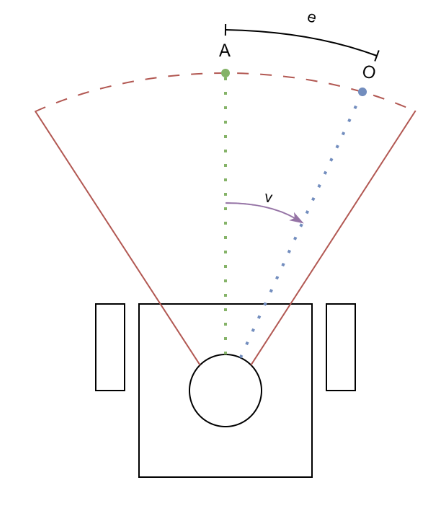
\includegraphics[width=6.5cm]{img/4_Implement/lane_keeping/top_down_view.png}
        \caption{Góc nhìn từ trên xuống}
    \end{subfigure}%
    \begin{subfigure}{0.6\textwidth}
        \centering
        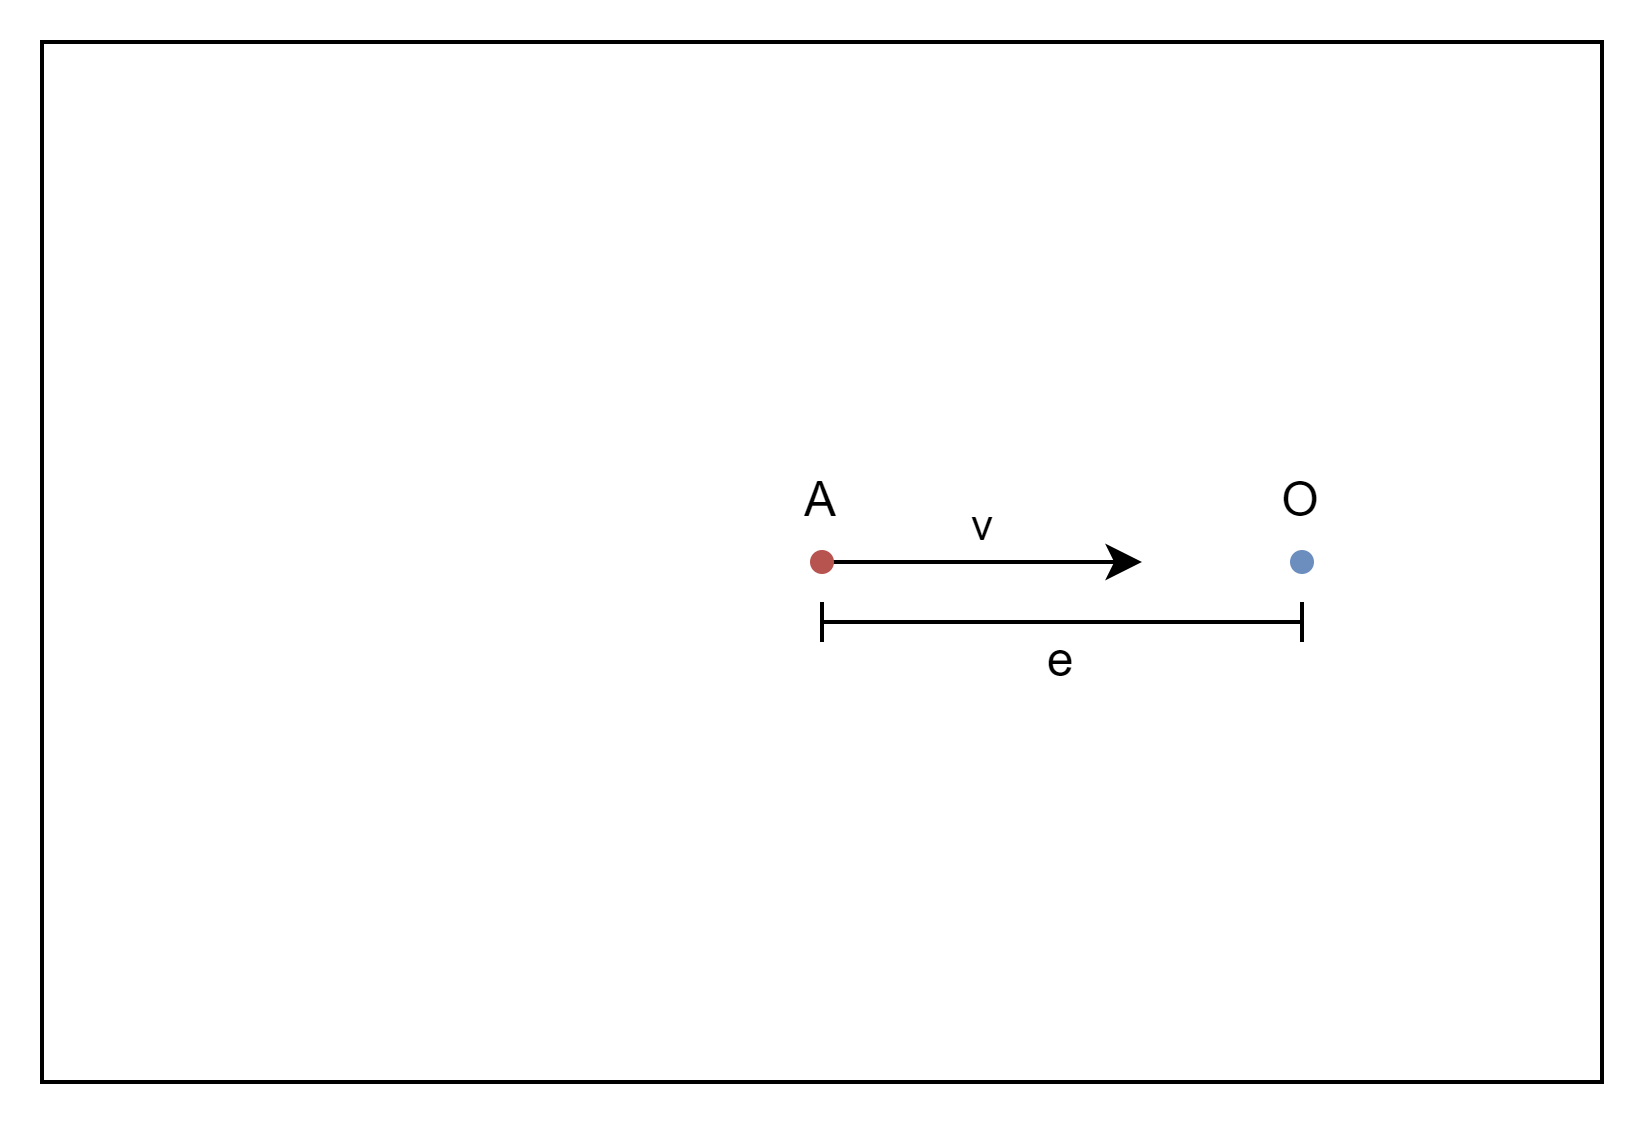
\includegraphics[width=8.5cm]{img/4_Implement/lane_keeping/camera_view.png}
        \caption{Góc nhìn camera}
    \end{subfigure}
    \caption{Minh họa điều khiển robot}
\end{figure}\\
\noindent Một điều rất tự nhiên, nếu vị trí hiện tại (điểm A) rất xa với vị trí mong muốn (điểm O), hay nói cách khác là sai số (error) lớn, ta cần điều chỉnh tốc độ xoay lớn để nhanh chóng đưa robot xoay đến vị trí O. Một cách đơn giản để công thức hoá lý tưởng này là dùng quan hệ tuyến tính:
\begin{equation}
    v = K_pe
\end{equation}
Trong đó $K_p$ là một hằng số dương mà ta gọi là hệ số P (Proportional Gain), $e$ là sai số cần điều khiển tức là khoảng cách từ điểm A tới điểm O. Mục tiêu điều khiển là đưa e tiến về 0 càng nhanh càng tốt. Rõ ràng nếu $K_p$ lớn thì $v$ cũng sẽ rất lớn và robot sẽ nhanh chóng xoay về vị trí O. Tuy nhiên khi đã đến vị trí O (tức $e = 0$), thì tuy vận tốc $v = 0$ nhưng do quán tính, robot vẫn tiếp tục xoay về bên phải và lệch điểm O về bên phải, sai số $e$ lại trở nên khác 0, giá trị sai số lúc này gọi là overshot (vượt quá). Lúc này, sai số $e < 0$, vận tốc $v$ sẽ xuất hiện với chiều ngược lại để kéo robot về điểm O. Nhưng một lần nữa, do $K_p$ lớn nên giá trị vận tốc $v$ cũng lớn và có thể kéo robot lệch về bên trái điểm O. Quá trính cứ tiếp diễn, robot cứ mãi dao động nhỏ dần quanh điểm O. Bộ điều khiển lúc này được nói là không ổn định.\\

\noindent Nhằm giảm overshot của robot, ta sẽ sử dụng một thành phần "thắng" trong bộ điều khiển. Sẽ rất lý tưởng nếu robot đang ở xa điểm O. Bộ điều sinh ra vận tốc $v$ lớn nhưng khi đã tiến gần đến điểm O thì thành phần "thắng" sẽ giảm tốc độ xoay của robot lại. Thành phần "thắng" này chính là thành phần D (Derivative), ta sẽ thu được bộ điều khiển PD như sau:
\begin{equation}
    v = K_pe + K_d\frac{de}{dt}
\end{equation}
Trong đó $\frac{de}{dt}$ là vận tốc thay đổi của sai số $e$ và $K_d$ là một hằng số dương gọi là hệ số D (Derivative Gain). Truy nhiên, trong đồ án này nhóm sẽ lược bớt thành phần I (Integral Gain), bộ điều khiển bây giờ sẽ là bộ điều khiển PD.\\

\noindent Có rất nhiều cách để chọn được thông số $K_p$ và $K_d$, nhóm sẽ chọn một cách thủ công bắt đầu từ $K_p = K_d = 0$, $K_p$ được tăng dần cho đến khi sai số $e$ bắt đầu dao động thì tăng $K_d$. Tại thời điểm $t = 0$, vị trí robot được thiết lập lệch khỏi làn đường là 80 ($e = 80$). Sau đó nhóm sẽ quan sát sự thay đổi của $e$ và đánh giá sự nhanh chóng, ổn định của bộ điều khiển.
\newpage
\begin{figure}[!hbt]
\begin{center}
    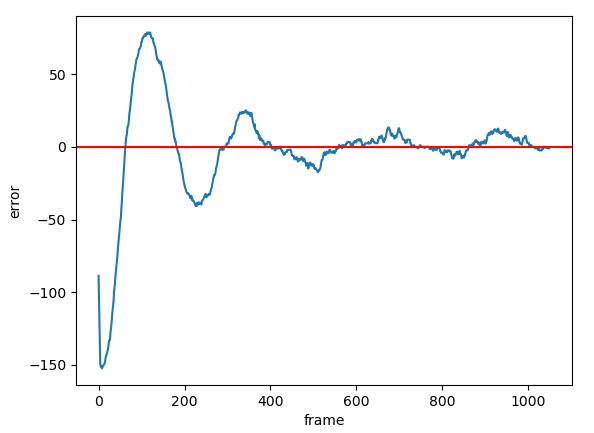
\includegraphics[width=12cm]{img/4_Implement/lane_keeping/error_plot.png}
    \caption{\label{pid_error_plot} Đồ thị sai số theo thời gian với $K_p = 0.0025, K_d = 0.007$}
\end{center}
\end{figure}
\noindent Có thể thấy ở hình \ref{pid_error_plot} có hiện tượng giống như overshoot, nhưng thực tế không phải là vậy. Nguyên nhân của hiện tượng này là do hiện tại robot đang được điều khiển thông qua tốc độ góc (angular\_z). Mặc dù tốc độ góc đang ở giá trị bằng 0, nhưng góc của robot vẫn có thể khác 0. Do robot luôn di chuyển theo hướng phía trước, khi góc của nó khác 0, robot sẽ đi chệch khỏi làn đường.
\begin{figure}[!hbt]
    \centering
    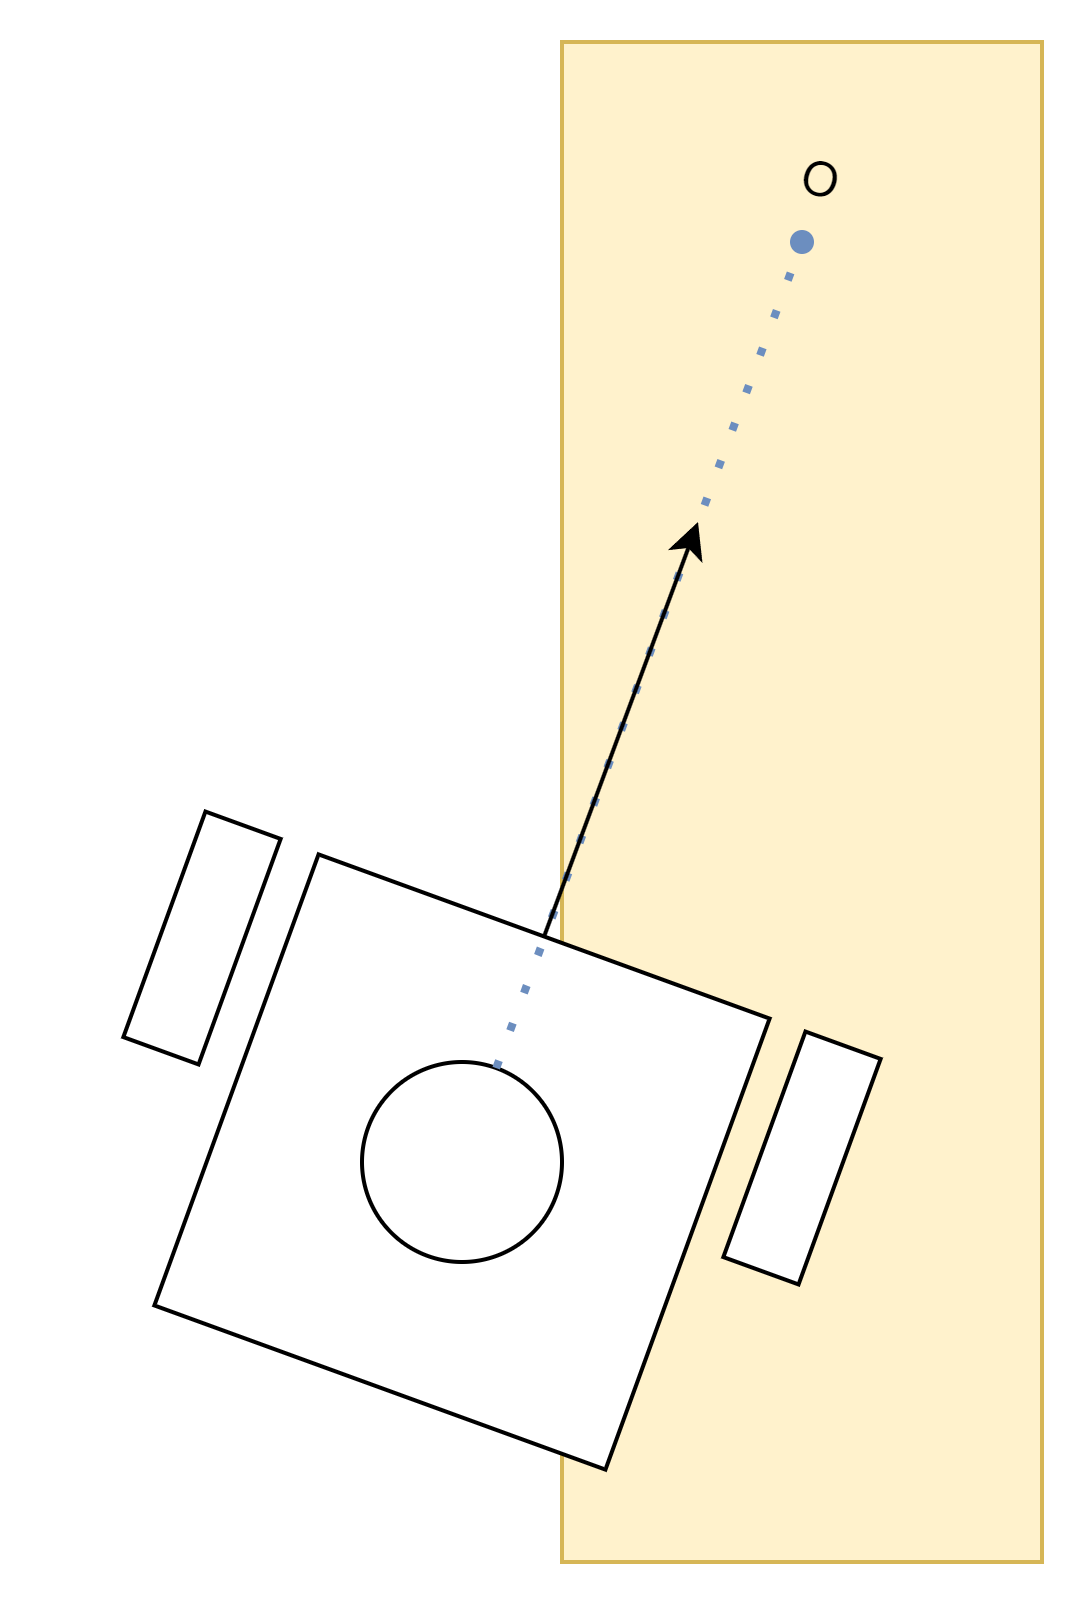
\includegraphics[width=5.5cm]{img/4_Implement/lane_keeping/error_view.png}
    \caption{Minh hoạ trường hợp đi lệch của robot}
\end{figure}